\PassOptionsToPackage{table}{xcolor}
\documentclass[american,titlepage,oneside]{ntnuthesis}
\setlength{\parindent}{15pt}

%define Javascript language
\lstdefinelanguage{JavaScript}{
keywords={typeof, new, true, false, catch, function, return, null, catch, switch, var, if, in, while, do, else, case, break},
ndkeywords={class, export, boolean, throw, implements, import, this},
sensitive=false,
comment=[l]{//},
morecomment=[s]{/*}{*/},
morestring=[b]',
morestring=[b]"
}

% Typescript
\lstdefinelanguage{Typescript}{
keywords={typeof, new, true, false, catch, function, return, null, catch, switch, var, let, const, if, in, while, do, else, case, break},
ndkeywords={class, export, boolean, throw, implements, import, this},
sensitive=false,
comment=[l]{//},
morecomment=[s]{/*}{*/},
morestring=[b]',
morestring=[b]"
}
 % Define new programming languages
\input{figures/diagram.tikzitstyles}

% Number subsubsections
\setcounter{tocdepth}{3}
\setcounter{secnumdepth}{3}

% Research questions
\newlist{questions}{enumerate}{2}
\setlist[questions,1]{label={\textbf{RQ\arabic*.}},ref={\arabic*},labelindent=\parindent,leftmargin=*,}
\setlist[questions,2]{label={--- \textbf{RQ\thequestionsi.\arabic*.}},ref={\thequestionsi.\arabic*},leftmargin=*}

\creflabelformat{questionsi}{#2\textup{#1}#3} % #2 and #3 are start and end of hyperlink.
\crefname{questionsi}{RQ}{RQs} % singular and plural forms of text labels
\Crefname{questionsi}{RQ}{RQs}
\creflabelformat{questionsii}{#2\textup{#1}#3}
\crefname{questionsii}{RQ}{RQs}
\Crefname{questionsii}{RQ}{RQs}
%

% FIXME: remove frontpage
\title{A Modeling Environment in the Cloud for
Education}
\shorttitle{Cloud Modeling for Education}
\author{Kristian Rekstad}
\shortauthor{K. Rekstad}
\date{\parbox{\linewidth}{\centering%
  {June~11,~2021}\endgraf\bigskip
  Master's Thesis\endgraf\medskip
  Dept.\ of Computer Science \endgraf{}
  Norwegian University of Science and Technology}}

\addbibresource{thesis.bib}

% Formatting help: 
% https://en.wikibooks.org/wiki/LaTeX/Text_Formatting#Hyphenation


% From https://www.overleaf.com/learn/latex/Glossaries

\makeglossaries % Prepare for adding glossary entries


%\newglossaryentry{latex}
%{
%        name=latex,
%        description={Is a mark up language specially suited for
%scientific documents}
%}

%\newglossaryentry{bibliography}
%{
%        name=bibliography,
%        plural=bibliographies,
%        description={A list of the books referred to in a scholarly work,
%typically printed as an appendix}
%}

\newglossaryentry{Theia}
{
  name=Theia,
  description={An \acrshort{IDE} for software development. Theia is accessible in a web browser and as a desktop application. The implementation reuses much of \gls{VSCode}'s internals. Managed by the Eclipse Foundation}
}

\newglossaryentry{VSCode}{
  name=VSCode,
  description={Visual Studio Code. An \acrshort{IDE} for software development. The full name is Visual Studio Code. Managed by Microsoft}
}

\newglossaryentry{metamodel}{
  name=metamodel,
  description={In conceptual modeling, the model itself can be modeled. This model of the model is called a meta-model. \Gls{Ecore} is one example of a metamodel}
}

\newglossaryentry{Ecore}{
  name=Ecore,
  description={The \acrshort{EMF} core model. A \gls{metamodel} similar to UML Class Diagrams}
}

\newglossaryentry{Eclipse}{
  name={Eclipse IDE},
  description={An \acrshort{IDE} by the Eclipse Foundation. Originally created by IBM. It is based on a plugin architecture using OSGi, and is written in Java}
}

\newglossaryentry{cloud}{
  name={cloud},
  description={Remote data centers that provide computing as a service. Commonly used by businesses to provide web infrastructure}
}

\newglossaryentry{open source}{
  name={open source},
  description={The source code for a software is available; not just for inspection, but for re-use and modification}
}

\newglossaryentry{Che}{
  name={Eclipse Che},
  description={A \gls{cloud} based or self hosted workspace and \acrshort{IDE} for software development. It is based on \gls{Kubernetes} and \gls{Theia}}
}

\newglossaryentry{GitHub}{
  name=GitHub,
  description={A website for software project management and source code sharing. Based on the Source-control Management (SCM) software called ``git'' }
}

\newglossaryentry{Gitpod}{
  name=Gitpod,
  description={A \gls{cloud} based workspace and \acrshort{IDE} for software development. It is based on \gls{Docker}, \gls{Kubernetes} and \gls{Theia}}
}

\newglossaryentry{Kubernetes}{
  name=Kubernetes,
  description={A container orchestration system created by Google}
}

\newglossaryentry{Docker}{
  name=Docker,
  description={A linux containerization system for process isolation and distribution. Popular for distributing and deploying self-contained software applications}
}

\newglossaryentry{UML}{
  name=UML,
  description={Unified Modeling Language. A common modeling language for creating diagrams such as Class Diagrams. It is standardized by \acrlong{OMG}}
}

\newglossaryentry{Electron}{
  name={Electron},
  description={A desktop application runtime for javascript, based on Chromium}
}
\newglossaryentry{Nodejs}{
  name={NodeJS},
  description={A javascript interpreter for desktop, based on the Chromium V8 javascript engine. It also includes some desktop \acrshortpl{API} like filesystem access}
}

\newglossaryentry{JSON-RPC}{
  name={JSON-RPC},
  description={Remote Procedure Call (RPC) protocol using Javascript Object Notation (JSON) serialization. It allows a process to execute functions in another process and obtain the results}
}

\newglossaryentry{JSON}{
  name={JSON},
  description={Javascript Object Notation. A serialization format for object structures}
}

\newglossaryentry{REST}{
  name=REST,
  description={Represential State Transfer (REST). A paradigm for creating HTTP \acrshortpl{API}, centered around resources}
}

\newglossaryentry{WebSocket}{
  name=WebSocket,
  description={A two-way communication protocol over TCP sockets made available for web browsers. It allows for a persistent and reusable connection which can send multiple messages, unlike regular HTTP requests. Commonly used to avoid polling over HTTP, or live updates of a website}
}

\newglossaryentry{NPM}{
  name={NPM},
  description={Node Package Manager (NPM). Hosts javascript packages online. Similar to Maven Central, but for javascript}
}

\newglossaryentry{TypeScript}{
  name={TypeScript},
  description={A programming language developed by Microsoft. It is a superset of the Javascript programming language, and adds static typing. TypeScript code is compiled to javascript, and can then run in a web browser or \gls{Nodejs}}
}

\newglossaryentry{ELK}{
  name={Eclipse Layout Kernel},
  description={Eclipse Layout Kernel (ELK) is a system for automatic diagram layout.~\cite{eclipsefoundationEclipseLayoutKernel} It positions nodes and edges for optimal viewing}
}

\newglossaryentry{React}{
  name=React,
  description={A javascript framework by Facebook for rendering views in HTML}
}

\newglossaryentry{domain}{
  name=domain,
  description={A phenomena in the real world or area of interest that must be analyzed to solve a problem. A domain is often abstracted to consist of entities, relations, processes and rules}
}

\newglossaryentry{TDT4250}{
  name={TDT4250},
  description={Advanced Software Design. A course at \acrshort{NTNU}. It runs during the autumn, and teaches computer science students concepts like \acrshort{MDD}, code generation, \acrshort{DSL} and dynamic component based systems}
}

%\newglossaryentry{API}{
%  name=API,
%  description={Application Programming Interface (API). The interface which  another program needs to use. This can be protocols and message contents, or  programming language constructs like function definitions}
%  long={Application Programming Interface},
%  first={\glsentrylong{api}} (\glsentryname{api})
%}

% --------------------
% ----- Acronyms -----
% --------------------

%\newacronym{phd}{PhD}{philosophiae doctor}
%\newacronym{CoPCSE}{CoPCSE@NTNU}{Community of Practice in Computer ScienceEducation at NTNU}
%\newacronym{gcd}{GCD}{Greatest Common Divisor}

\newacronym{MDD}{MDD}{Model-Driven Development}
\newacronym{IDE}{IDE}{Integrated Development Environment}
\newacronym{EMF}{EMF}{Eclipse Modeling Framework}
\newacronym{NTNU}{NTNU}{Norges Teknisk-naturvitenskapelige Universitet}
\newacronym{API}{API}{Application Programming Interface}
\newacronym{DSL}{DSL}{Domain-specific language}
\newacronym{OCL}{OCL}{Object Constraint Language}

\newacronym{EMOF}{EMOF}{Essential Meta Object Facility}
\newacronym{OMG}{OMG}{Object Management Group}
\newacronym{XMI}{XMI}{XML Metadata Interchange}

\newacronym{RCP}{RCP}{Rich Client Platform}
\newacronym{RAP}{RAP}{Remote Application Platform}
\newacronym{GWT}{GWT}{Google Web Toolkit}

\newacronym{LSP}{LSP}{Language Server Protocol}
\newacronym{GLSP}{GLSP}{Graphical Language Server Platform}
\newacronym{RPC}{RPC}{Remote Procedure Call}

\newacronym{svg}{svg}{Scalable Vector Graphics}
 % add glossary and acronym lists before document

\begin{document}
\chapter*{Abstract}

% TODO
\chapter*{Sammendrag}

Programvareutvikling har en tilnærming som kalles Model-Dreven Utvikling (MDD).
Dette undervises til studenter i høyere utdanning.
Tilnærmingen er avhengig av verktøy, og et slikt verktøy er Eclipse Modeling Framework (EMF).
Selv om EMF kan brukes for å lære studenter om MDD, er det upopulært på grunn av sin tilknytning til Eclipse Integrated Development Environment (IDE), som gjør at studenter stritter i mot å lære MDD.
Skybaserte alternativer til Eclipse IDE eksisterer, som Gitpod med VSCode, og de har nyttige egenskaper for en utdanningsorganisasjon.
Verktøyene i EMF finnes derimot ikke for disse alternativene.
Denne masteroppgaven prøver å legge til rette for å støtte EMF i de skybaserte alternativene.

Fremgangsmåten i masteroppgaven er basert på Design Science Research, hvor et design blir lagd og en programvare blir utviklet.
Designet drar inspirasjon fra Language Server Protocol (LSP) og Graphical Language Server Platform (GLSP), protokoller for tekst- og diagramredigering.
Disse protokollene brukes allerede i VSCode.

Resultatet er en utvidelse for VSCode for redigering av tre-strukturer.
EMF-modeller kan redigeres som trær.
Denne utvidelsen består av tre komponenter: et generisk brukergrensesnitt for tre-redigering, en utvidelse for VSCode, og en EMF-spesifikk tjener (server).
Utvidelsen og serveren snakker med en nylig designet protokoll: \acrfull{TLSP}.

Den resulterende programvaren kan bygges på videre, for å bruke EMF-modellering i skyen.
TLSP-protokollen og programvarearkitekturen kan brukes av også andre verktøy som trenger tre-redigering, og som sikter på å støtte flere IDE-er.
En utbredt bruk av TLSP i IDE-er vil gjøre at migrering av tre-redigeringsverktøy til andre IDE-er blir forenklet.
Uavhengig av dette, så gir designet en gjenbrukbar server for EMF, som kan forenkle migreringen av EMF til andre IDE-er.
\cleardoublepage{} % Force odd-numbered page.
\chapter*{Acknowledgments}

\paragraph*{Hallvard Trætteberg} for being a very helpful supervisor
and for interesting discussions.

\paragraph*{Norwegian University of Science and Technology (NTNU)} for providing access to research papers, my education, and for providing an office to write this thesis. 

\paragraph*{Dr.\ Jonas Helming and Maximilian Koegel} at EclipseSource for their helpful blog posts. An Dr.\ Helming in particular, for providing answers about my research at the EclipseCon 2020 conference, and the initial title for the thesis.

\paragraph*{COPCSE-NTNU} for this latex document template: \href{https://github.com/COPCSE-NTNU/thesis-NTNU}{https://github.com/COPCSE-NTNU/thesis-NTNU}.

\paragraph{Abakus, Online and TIHLDE student organizations} for free coffee, and for selling noodles and candy.

\paragraph{My parents Jenny and Håvard, and Ingrid M. J.} for all the love, support and motivation they give me.

% Emf.cloud and glsp developers
% Vscode developers
% LSP designers

% Melanie Bats
% Philip Langer

% Ingrid?
% Mom & Dad
 

\tableofcontents
\listoffigures
\listoftables
\lstlistoflistings{}

\printglossary[type=\acronymtype] % Print acronyms
\printglossary{}                    % Print glossary


\chapter{Introduction}\label{chap:introduction}

\section{Model-Driven Development in Education at NTNU}
% * NTNU, TDT4250, EMF in education, Eclipse IDE for EMF, shift from Eclipse to web with Theia/VSCode

\paragraph{In a world that becomes more digital for each day, there is a large need for software development.} Software is often created by writing code using programming languages that compile down to computer instructions. Developers write the code based on a set of requirements, and change it when the  requirements change.

\paragraph{One alternative approach to software development, is \acrfull{MDD}.}
This approach has the developers create models of their \gls{domain}, and this model drives the rest of the software development. 
The code is usually generated from the model. 
If the software requirements change, the model is updated first, and the code is re-generated.
The model itself is often one or more artifacts in the software project, expressed in a modeling language.
Modeling simplifies the \gls{domain} by using abstraction, and reduces the world down to the entities, relations, procedures (or other abstractions) that are needed to solve the relevant problems.


\paragraph{The \acrshort{MDD} approach is taught at \acrfull{NTNU}.}
The course is named \textit{\gls{TDT4250} Advanced Software Design}.
A modeling language called \textit{\gls{Ecore}} is used in \gls{TDT4250}.
This language comes from the \acrfull{EMF}.
The models can generate java code, and can extend the \gls{Eclipse} as a plugin.
The plugin lets a user enter data for a model instance by using \gls{Eclipse} as a user interface.
Students also learn to create \acrfullpl{DSL} with an \gls{Ecore} model as its core.

\paragraph{\Gls{Eclipse} is required to work with \acrshort{EMF} modeling.}
It has editors for \gls{Ecore}, code generation and model validation.
There are two main types of editors: hierarchical tree editors and graphical diagram editors.
There are also multiple different implementation on the tree editors, based on different underlying frameworks.

\paragraph{The reliance on \gls{Eclipse} is a problem for students.}
Students don't like to work in Eclipse, because of various issues with usability, errors or stability. %TODO: cite?
If a student wants to use \acrshort{EMF} afterwards in their job, they would have to use \gls{Eclipse}, and also convince their team to do it as well.
Some students see \acrshort{EMF} as being too \gls{Eclipse} related, as well, and incorrectly see it as a tool for only developing Eclipse plugins.
This results in students resisting to learn \acrshort{EMF}, and also \acrshort{MDD} by implication, because no \acrshort{EMF} alternative is taught.

\paragraph{\acrshort{NTNU} wants to move from \gls{Eclipse} to \gls{VSCode} running in a web browser.}
This is a recent decision, and mainly for the course in Object Oriented Programming with java.
Some of the reasoning behind the change, is to avoid installation issues from \gls{Eclipse}, and to ease online collaboration through \gls{GitHub} and publication of assignments. %TODO: cite?
\gls{VSCode} is an advanced text editor that has increased in popularity in the recent years.
It is based on web technologies, but normally runs as a desktop application.
A website and service called \textit{\gls{Gitpod}} allows running \gls{VSCode} in a web browser, and connect it to a workspace based on a \gls{GitHub} repository.
The workspace has the project files, software development kits and other tools already installed and running in a remote machine in the \gls{cloud}.
This avoids all installation on a student's machine.

\paragraph{For \gls{TDT4250} to follow suit and move to \gls{Gitpod}, the \gls{Ecore} editors would have to be available in \gls{VSCode} as well.}
The current situation is that there are no \gls{Ecore} editors for \gls{VSCode}.
There are also no known \acrshort{MDD} frameworks for \gls{VSCode} that integrates with the other curriculum of \gls{TDT4250} either, as alternatives to \acrshort{EMF}.


\section{The Eclipse Ecosystem Wants to Run Software in the Cloud}
%* Eclipse ecosystem is moving to the cloud, EMF.Cloud, GLSP, Theia, Gitpod, Sprotty.
%  * Pre-project identified that the main actors are TypeFox, EclipseSource, RedHat, Obeo
%  * Main focus on development, not the developer; code in Eclipse and run in cloud

\paragraph{The \acrlong{EMF} is powered by \gls{open source} software and an ecosystem of developers.}
The framework has many tools and software libraries available, contributed by various developers and organizations.
These developers and organizations, is what this thesis nicknames the \textit{Eclipse Ecosystem}.
Some prominent actors are the organizations \textit{TypeFox}, \textit{EclipseSource} (with Dr.\ Jonas Helming and Maximilian Koegel), \textit{Obeo} and \textit{RedHat}~\cite{rekstadModelingEnvironmentCloud2020}.
For example, \textit{\gls{Gitpod}} is developed by TypeFox, and one of the \gls{Eclipse} tree editors for \gls{Ecore} is created by EclipseSource~\cite{typefoxTypeFoxSmartTools,eclipsesourceEMFFormsEditors2016}.

\paragraph{\Gls{cloud} is becoming more popular, and the Eclipse Ecosystem is heading there.}
When something \textit{runs in the \gls{cloud}}, it really means that it runs on rented computers in a data center somewhere outside of the organization.
Running in the cloud is a win for developers and organizations, because they don't need to take care of their own hardware.
And scaling up to more computers is as easy as clicking a button, or often happens automatically with load balancing technology.
No more purchasing of hardware and configuring it.
When developers ``embrace'' the \gls{cloud}, it also means working more with web technologies and less with desktop applications.

\paragraph{To use \acrshort{EMF} in the cloud, the Eclipse ecosystem has started to create new tools.}
Most of the tools are related to \textbf{running} \acrshort{EMF}-based software, but not \textbf{developing} it.
There are \textit{some} advances to developing in the cloud, with \textit{Gitpod} and the \gls{VSCode} re-implementation \textit{\gls{Theia}}, but neither have tools for \acrshort{EMF}.


\section{A Pre-project Identified a Need for a Tree Editor}
% EclipseCon, GLSP, Ecore GLSP, Theia extension, Gitpod, 

\paragraph{This masters thesis is preceded by a pre-project thesis.}
This work happened during the Autumn of 2020, the semester before this masters thesis.
The results were presented in \cite{rekstadModelingEnvironmentCloud2020}.
The project began by identifying what to build.
The need for \acrshort{EMF} editing in the \gls{cloud} was known, but not how to do it or if it was even possible.

\paragraph{The pre-project identified a need for a web-based tree editor for working with \acrshort{EMF}.}
Early plans were to create a diagram editor, inspired by \textit{\gls{UML} Class Diagrams} and the \gls{Eclipse} diagram editor for \gls{Ecore} named \textit{Ecore Tools} (based on \textit{Sirius} by aforementioned Obeo)~\cite{rekstadModelingEnvironmentCloud2020}.
During an online conference for the Eclipse ecosystem, EclipseCon 2020, it became clear that EclipseSource was already working on this~\cite{jonashelmingEcoreToolsCloud2020}.
However, based on the author's experience as a former student of \gls{TDT4250}, most of the work with \gls{Ecore} happened in a tree structure\footnote{\textit{Tree structure} here means the hierarchical parent-child structure, perhaps better known from file system folders and file browsers.} editor with a property sheet.
This kind of editor has what is known as a \textit{master-detail layout}, where the tree is a master view, and the property sheet is the details of the current selection in the tree.
No actor in the Eclipse ecosystem was working on such a tree editor for \gls{Ecore} models for \gls{VSCode}.
Preliminary searches online did not find such an editor created by anyone outside the Eclipse ecosystem either.

% TODO: add a picture of a tree editor

\paragraph{Initial requirements for a tree editor were chosen.}
The period of work was constrained to the pre-project and master's thesis, which is from August 2020 to June 2021.
This constraint made it a goal to reduce the amount of unnecessary work and reduce re-implementation of existing solutions.
For example, the \acrlong{EMF} is big, with many years worth of experience ingrained in its implementation details.
Therefore, a non-functional requirement emerged: \textbf{the editor should re-use as much of the existing \acrshort{EMF} java code as possible.}


Another non-functional requirement was that \textbf{it should run inside \gls{VSCode} as an extension}.
Gitpod was at the time was using \gls{Theia} as the editor, which was compatible with \gls{VSCode} extensions~\cite{rekstadModelingEnvironmentCloud2020}.
\Gls{Theia} has two extension mechanisms, but only the \gls{VSCode} extension mechanism could be installed during runtime by students~\cite{rekstadModelingEnvironmentCloud2020}.
Because a goal was to use the Gitpod service for \gls{TDT4250}, this compatibility was needed.


The third non-functional requirement was that \textbf{the project should be \gls{open source} and designed to live longer than the period of work.}
A goal is to include all or most of the functionality already present in \gls{Eclipse}, which was estimated to be more work than what was possible to do during the pre-project and master's thesis.
Therefore, the development will need to be taken over by someone else afterwards.
Either the Eclipse ecosystem, or a master's thesis by another student.
An \gls{open source} project needs some additional care if it wants to succeed.
For the Eclipse ecosystem to handle it, the software should have a compatible license, and not copy or use code with incompatible licenses.
The code should also be well structured, documented and easy to contribute to for others.


The initial, unrefined functional requirement was that \textbf{\gls{VSCode} should be able to view, edit and save \gls{Ecore} models and model instances in ``.ecore'' and ``.xmi'' files.}
The pre-project did further work to refine this functional requirement into multiple smaller requirements, and discovered many new ones, by requirements extraction~\cite[p.~47,48]{rekstadModelingEnvironmentCloud2020}.
As noted in the discussion in \cite[p.~51]{rekstadModelingEnvironmentCloud2020}, the list of functional requirements was not complete.
% TODO: add requirements as appendix?


\paragraph{A software architecture and protocol emerged by analyzing similar solutions.}
Because the \acrshort{EMF} tooling had to move to \gls{VSCode} now, it is plausible that it will need to move to another \acrshort{IDE} later in the future.
This could result in a customized plugin for each editor.
That problem is also seen in programming languages: every editor needs a plugin for every programming language.
Microsoft has tried to solve this combinatorial ``\(m{\times}n\)'' problem in \gls{VSCode} by introducing the \acrfull{LSP}.
This architecture was also used as inspiration for a Eclipse ecosystem project, the \acrfull{GLSP}.
A similar protocol design could benefit this tree editor, where the \gls{Ecore} language details are isolated in a component reusable across \acrshortpl{IDE}~\cite{rekstadModelingEnvironmentCloud2020}.


The architecture was also inspired by \acrshort{GLSP} in terms of components for the \gls{VSCode} extension.
A ``generic'' frontend that handles all kinds of tree structures is hosted in a webview inside \gls{VSCode}, and talks to the \gls{VSCode} extension.
The extension code bridges the \gls{Ecore} specific server to the generic frontend via the previously mentioned protocol~\cite{rekstadModelingEnvironmentCloud2020}.

% TODO: add figure of architecture?

\paragraph{The pre-project used prototypes to verify the feasibility of the architecture.}
The main issues solved in the pre-project were related to design choices and feasibility.
It tried to answer if and how such a \gls{Ecore} specific server could be made in java and be executed from the \gls{VSCode} extension itself.
The pre-project also looked for a good data model to support editing of any tree structure, while providing a user interface with high usability and constraints~\cite[p.~24,25]{rekstadModelingEnvironmentCloud2020}.

\paragraph{More work was needed in order to evaluate the pre-project solution.}
No complete editor was produced during the pre-project.
Its feasibility was confirmed through several prototypes, however, and a minimal implementation was made.
This implementation was not completed to the point where it could establish a protocol between the extension and \gls{Ecore} server.
It could only render an example tree in \gls{VSCode} and \gls{Theia} in \gls{Gitpod}.
This master's thesis will pick up on these results and try develop them further into a usable solution.
It also aims to create an \gls{open source} repository that is viable and suitable for further development by the Eclipse ecosystem and other master students.

\section{Research Objectives}

\subsection{Problem}

\paragraph{Problem definition}
How can students use the \acrfull{EMF} in a \gls{cloud} based \acrfull{IDE} in order to learn \acrfull{MDD} as part of the course \gls{TDT4250}, \textit{without} using the \gls{Eclipse}?

\paragraph{Value}
\begin{enumerate}
  \item Students may be more motivated to learn \acrshort{MDD} if they do not need to use \gls{Eclipse}, and do not perceive the \acrshort{MDD} framework (\acrshort{EMF}) as \gls{Eclipse}-specific or only for deploying to the \gls{Eclipse}~\cite[p.~2]{rekstadModelingEnvironmentCloud2020}.
  Few to no other courses at \acrshort{NTNU} target \gls{Eclipse} as the deployment/target platform, and \textcite{kuzniarzTeachingModelDrivenSoftware2016} found that students resist learning when the technology and skills are not used in other courses.
  Students also dislike or have problems with \gls{Eclipse} itself, and feedback collected from teaching students in 2015 by \textcite{jordicabotFailedConvinceMy2015} found that much of the complaints were about installation issues and problems with the tools, not problems with \acrshort{MDD} as a concept.
  
  \item By moving \acrshort{EMF} from \gls{Eclipse} to other \gls{IDE}, the value of the framework itself may increase, as adoption of \acrshort{EMF} does not imply adoption or use of \gls{Eclipse}.
  Industry may use the framework for modeling, without requiring the developers to use \gls{Eclipse}.
  A problem for \acrshort{MDD} adoption in general is low impact on personal career needs, identified by \textcite{jonwhittleTaxonomyToolrelatedIssues2015}.
\end{enumerate}
  

\subsection{Objectives}

There are two objectives for this thesis.

\paragraph{Objective 1: EMF Modeling in the Cloud}
The first objective is to perform \acrfull{MDD} by using \acrfull{EMF} in a cloud based \acrshort{IDE}.
\Gls{Gitpod} with \gls{Theia} is chosen as the \acrshort{IDE}.
A solution should be able to perform all the tasks needed to teach \acrshort{MDD}, and \gls{Eclipse} should not need to be installed on a student's computer.

\paragraph{Objective 2: Open Source project}
The artifact should exist longer than the period of work for the master's thesis, and be developed further by contributors other than this thesis' author.
The artifact should be in a \gls{open source} project, to fit in with the expectations of the Eclipse ecosystem, current trends and expectations of students.

% Thesis structure ?
%TODO
\chapter{Background}\label{chap:background}

This background section will explain some of the concepts, approaches, technologies and software architectures required to understand this thesis.
The findings from the pre-project in \cite{rekstadModelingEnvironmentCloud2020} will also be presented in more detail than the introduction, as the findings are central to this thesis.
Lastly, a section on open source software project management follows, as they shape many of the choices made in the implementation of a solution.

\section{Conceptual Modeling and Model-Driven Development}\label{sec:conceptual-modeling}

\paragraph{Rationale}
\Acrfull{MDD} is the approach to software development which this thesis aims to support.
Therefore, and understanding of \acrshort{MDD} is beneficial, in order to see how an editor should work.

\paragraph{Modeling and abstraction}
The core of \acrshort{MDD} is the model.
The model is a human created construct, formed through humans working together to discuss and refine a problem domain until they reach a consensus of what abstractions help them solve the relevant problems~\cite[p.~154]{brambillaModeldrivenSoftwareEngineering2012}.
Humans perceive the world (and problem domain) as many different phenomena, and conceptual modeling is the act of trying to describe these at some level of abstraction~\cite[p.~1,408]{krogstieModelbasedDevelopmentEvolution2012}.
The model is assumed to resemble the phenomena and work the same way, and yet be simpler than the real world~\cite[p.~414]{krogstieModelbasedDevelopmentEvolution2012}.
Abstraction means to find something common in different observations of a phenomena, and \textit{generalize} their features, \textit{classify} coherent clusters of objects and \textit{aggregate} concepts into more complex ones~\cite[p.~1]{brambillaModeldrivenSoftwareEngineering2012}.
The model will never describe every aspect of the world perfectly, but can \textit{reduce} the world down to relevant aspects, and easily \textit{map} between model elements and real world phenomena~\cite[p.~1-2]{brambillaModeldrivenSoftwareEngineering2012}.


\paragraph{Modeling languages}
In order to describe the model, a \textit{language} is used.
To realize the benefits of \acrshort{MDD}, a \textit{formal language} is used.
The language can be textual or graphical, or both, and imposes a formally defined syntax on the modeler~\cite[p.~13]{brambillaModeldrivenSoftwareEngineering2012}.

\paragraph{Modeling tools}
The advantage of using a formal language is that it can be parsed and understood by software tools, as well as humans.
The tools can validate the model according to the syntax, and to specific rules for the domain.
Tools can also generate code, or execute the model itself.
The model can be transformed into other models, or text or graphics~\cite[p.~8]{brambillaModeldrivenSoftwareEngineering2012}.

\paragraph{\acrlong{MDD}}
The central idea of \acrlong{MDD} is that the model is the source of truth that \textit{drives} the rest of the engineering and development~\cite[p.~9]{brambillaModeldrivenSoftwareEngineering2012}.
There is not a separate model for analysis and for design, but a single one for both~\cite[p.~49]{evansDomaindrivenDesignTackling2004}.
The software code becomes an expression of the model itself, and changes to the code often happen as the result of changes to the model~\cite[p.~49]{evansDomaindrivenDesignTackling2004}.
Because the model and the software are so directly related, the \acrshort{MDD} approach is heavily reliant on tools to automate the tasks of validation and code generation.
The formal language may also sacrifice some of its human readability in order to be understood by tools~\cite[p.~232]{krogstieModelbasedDevelopmentEvolution2012}.
To solve this, one can use other tools that interpret, transform or present models in other ways~\cite[p.~233]{krogstieModelbasedDevelopmentEvolution2012}.
This increases the reliance on tools for \acrshort{MDD} even more, including visual editors.




\section{Model-Driven Development at NTNU in the Course TDT4250}\label{sec:tdt4250}
% * TDT4250. Modeling, use of instances to validate model as you develop, validation of models.

\paragraph{Rationale}
Because the target audience of the software solution (tree editor) are students at \acrshort{NTNU}, it is helpful to know how they work with \acrlong{MDD}.
Their use cases are the ones being solved, meaning the solution must be made with this context in mind.

\paragraph{\Acrshort{MDD} at \acrshort{NTNU}}
To do \acrlong{MDD} effectively, tools should be used.
In the course ``\textit{\gls{TDT4250} Advanced Software Design}''\footnote{Course description is available at \href{https://www.ntnu.edu/studies/courses/TDT4250\#tab=omEmnet}{https://www.ntnu.edu/studies/courses/TDT4250\#tab=omEmnet}.} at \acrshort{NTNU}, the chosen tools are in the \acrfull{EMF}~\cite{hallvardtraettebergEMFTDT4250NTNU2017}.
This includes the modeling language \gls{Ecore}, visual editors in \gls{Eclipse}, model validation logic, the code generator named ``GenModel''\footnote{The code generator is actually named ``codegen'', but users only see the configuration model called ``GenModel''.} (generator model), and more.
\Acrshort{EMF} is a battle-tested technology also used in certain industries, and is well integrated with the \gls{Eclipse}.
The course \gls{TDT4250} also uses \gls{Eclipse} as a case study for other software design concepts, such as modularity (plugin architecture) and dynamic systems (OSGi), and custom \acrlongpl{DSL} which automatically work with \gls{Eclipse}.
\Acrshort{EMF} is relevant for most or all of those concepts.

\paragraph{Development methodology}\label{par:tdt4250-methodology}
Students are taught a methodology or approach for how to do modeling.
They start by specifying a problem space, for example bookkeeping an organization of employees or the courses in \acrshort{NTNU}, and then abstract the problem into a model.
The initial model is externalized as \gls{Ecore} by using a tree editor in \gls{Eclipse}.


Then an \textit{model instance} is made, based on the model, and filled with example data from the domain.
This model instance is used to test and verify that the model is appropriate for the problem space.
Adjustments are made to the model to accommodate any problems with the model instance.


Then validations can be created for the model, by one or both of the following approaches: writing \acrfull{OCL} into model annotations, or marking the model element with an annotation and implementing it as java code.
\Acrshort{OCL} is a \acrlong{DSL} for navigating models and evaluating expressions, and the \gls{Eclipse} can detect annotations with \acrshort{OCL} and evaluate them against the \gls{Ecore} model.
The other option, writing java code, requires the student to first create a new \textit{genmodel} file from the model (by using a menu in \gls{Eclipse}), generating a java code project from the model, and then writing validation logic into the generated code.
For the java code to be picked up, \gls{Eclipse} can start a new instance which installs the generated code as a plugin~\cite{hallvardtraettebergConstraintsValidationTDT42502020}.


Next up, when the model is deemed sufficient, and the most important validations are in place, the student can try to create a user interface.
One of several choices here is to create an \textit{\gls{Eclipse} plugin}.
\Acrshort{EMF} provides code generation for utilities used to integrate the model into an editor for \gls{Eclipse}.
The student uses the genmodel to create these, and tweaks the code if wanted.
Then everything is installed into \gls{Eclipse} by launching a new \gls{Eclipse} instance with the code installed as a plugin.


Lastly, the user interface can be tested.
The student creates a new model instance file, enters some example data from the domain, and runs validation logic.

\paragraph{Lecture materials}\label{par:tdt4250-confluence}
The steps mentioned in the methodology above are available online in \cite{hallvardtraettebergEMFStepbystepTDT42502017,hallvardtraettebergConstraintsValidationTDT42502020,hallvardtraettebergEditingEcoreModel2017,hallvardtraettebergGenmodelTDT4250NTNU2017}.
This is an advantage, because they can by used used in this master's thesis as a basis for creating evaluations and acceptance criteria.



\section{Eclipse Modeling Framework Editors for Ecore}\label{sec:emf-editors}

\paragraph{Rationale}
These editors are the ones being re-implemented in \gls{cloud}-based \acrshortpl{IDE}.
Understanding their functionality and workings is important, as these editors shape the work of this thesis.
The functionalities provided are assumed highly usable and good, because they are the result of many years of work and experience.
This allows this thesis to skip the work of doing usability testing with regards to feature design, as long as the features are similar enough to the copied ones.

\paragraph{Multiple editors}
When editing \gls{Ecore} models in \gls{Eclipse}, there are different editors to pick from.
Usually, \gls{Ecore} models and model instances are saved as \acrfull{XMI}, which is a standardized serialization format based on XML.
The \gls{Ecore} models have the file extension \texttt{.ecore} while model instances either have \texttt{.xmi} or a custom extension for the model, specified by the modeler (e.g. \texttt{.organization} or \texttt{.courses}).
The GenModel has \texttt{.genmodel} as file extension.
However, \gls{Ecore} models are rarely (if ever) edited as XML.
Instead, the files are loaded and presented in a tree structure editor or diagram editor.
These editors are specialized for \gls{Ecore}, and can understand the model.


The diagram based editors use a notation that is based on \gls{UML} Class Diagrams, with boxes, labels and arrows.
Which editor to use can often be a personal preference.
They are all functionally equivalent, with regards to modeling.
The next subsections will describe the most common tree editors in more detail.

\subsection{Sample Reflective Ecore Model Editor}\label{sec:sample-reflective-editor}

The ``\textit{Sample Reflective Ecore Model Editor}'' is one of the main \gls{Ecore} editors in \gls{Eclipse}.
A screenshot of the editor is shown in \cref{fig:sample-reflective-ecore-model}.
The model instances can be edited in a \textit{reflective} editor (without the user first generating java code and installing an \gls{Eclipse} plugin).
Here, reflective means that the editor uses a metamodel (see \cref{sec:emf-metamodel}) for the model instance, and tries to infer the tree structure from containment relationships.


This editor can open both \gls{Ecore} models and model instances.
A screenshot of a model opened in the editor is shown in \cref{sfig:sample-reflective-ecore-model-screenshot}, and a model instance in \cref{sfig:sample-reflective-ecore-model-instance-screenshot}.


This editor is \gls{open source}%
\footnote{Sample Reflective editor source: \href{https://git.eclipse.org/c/emf/org.eclipse.emf.git/tree/plugins/org.eclipse.emf.ecore.editor}{\nolinkurl{https://git.eclipse.org/c/emf/org.eclipse.emf.git/tree/plugins/org.eclipse.emf.ecore.editor}}.}%
, and the editor is itself originally generated by a genmodel~\cite[p.~10]{rekstadModelingEnvironmentCloud2020}.


This editor internally uses a java class called \texttt{ReflectiveItemProvider}%
\footnote{\texttt{ReflectiveItemProvider} source code: \href{https://git.eclipse.org/c/emf/org.eclipse.emf.git/tree/plugins/org.eclipse.emf.edit/src/org/eclipse/emf/edit/provider/ReflectiveItemProvider.java}{\nolinkurl{https://git.eclipse.org/c/emf/org.eclipse.emf.git/tree/plugins/org.eclipse.emf.edit/src/org/eclipse/emf/edit/provider/ReflectiveItemProvider.java}}}
from the \texttt{org.eclipse.emf.edit} \acrshort{EMF} package, to extract text labels and infer icons for the tree view~\cite[p.~10]{rekstadModelingEnvironmentCloud2020}.


For \gls{Ecore} models (with \texttt{.ecore} file extension, not model instances), it uses an \texttt{EcoreItemProviderAdapterFactory}%
\footnote{\texttt{EcoreItemProviderAdapterFactory} source code: \href{https://git.eclipse.org/c/emf/org.eclipse.emf.git/tree/plugins/org.eclipse.emf.ecore.edit/src/org/eclipse/emf/ecore/provider/EcoreItemProviderAdapterFactory.java}{\nolinkurl{https://git.eclipse.org/c/emf/org.eclipse.emf.git/tree/plugins/org.eclipse.emf.ecore.edit/src/org/eclipse/emf/ecore/provider/EcoreItemProviderAdapterFactory.java}}}
to get labels and icons~\cite{edmerksEcoreEditorJava2021}.


These ``item providers'' are especially interesting, because they could be reused in a new editor.

\begin{figure}
    \centering
    \begin{subfigure}[b]{.45\textwidth}
        \centering
        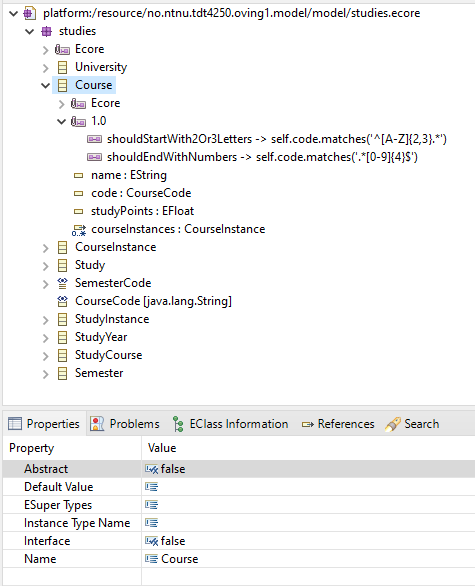
\includegraphics[width=\textwidth]{figures/pre-project/ecore-sample-reflective-ecore-model-editor}
        \caption{A model opened in the editor.}\label{sfig:sample-reflective-ecore-model-screenshot}
    \end{subfigure}
    \hfill
    \begin{subfigure}[b]{.45\textwidth}
        \centering
        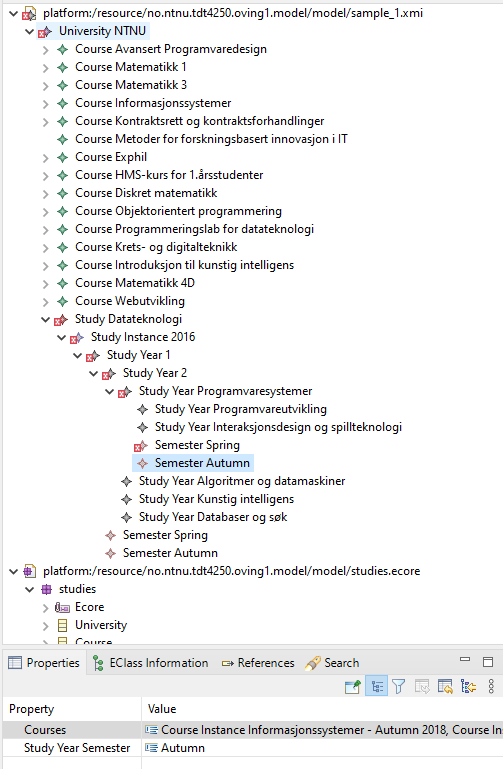
\includegraphics[width=\textwidth]{figures/pre-project/ecore-sample-reflective-ecore-model-editor-instance.png}
        \caption{A \emph{dynamic instance} (\acrshort{XMI} file) opened in the editor.}\label{sfig:sample-reflective-ecore-model-instance-screenshot}
    \end{subfigure}
    \caption{Screenshots of the Sample Reflective Ecore Model Editor in \gls{Eclipse}.}\label{fig:sample-reflective-ecore-model}
\end{figure}


\subsection{EMF Forms Ecore Editor}\label{sec:emfforms-editor}

The \textit{EMF Forms Ecore Editor} is a newer editor than the Sample Reflective editor, and uses EMF Forms\footnote{More info about EMF Forms here: \href{https://www.eclipse.org/ecp/emfforms/index.html}{\nolinkurl{https://www.eclipse.org/ecp/emfforms/index.html}}.} as the technology to provide a user interface~\cite{eclipsesourceEMFFormsEditors2016}.
This editor is \gls{open source}%
\footnote{\textit{EMF Forms} source code: \href{https://git.eclipse.org/c/emfclient/org.eclipse.emf.ecp.core.git/tree/bundles/org.eclipse.emfforms.editor.ecore}{\nolinkurl{https://git.eclipse.org/c/emfclient/org.eclipse.emf.ecp.core.git/tree/bundles/org.eclipse.emfforms.editor.ecore}}.}.
A screenshot of the editor is shown in \cref{fig:emf-forms-ecore-editor}.


This editor is implemented as a generic editor for all \gls{Ecore} model instances, and two subclasses that are specialized for \gls{Ecore} and GenModel~\cite{eclipsesourceEMFFormsEditors2016}.
The generic editor is called \textit{Generic XMI Editor} in \gls{Eclipse}, and the \gls{Ecore} specific editor is called \textit{Ecore Editor}.


The biggest difference compared to the Sample Reflective editor, is how the user interface looks, and that the property sheet is customized based on a \textit{view model file}.
The Sample Reflective editor uses \gls{Eclipse}'s built in property panel.
In the EMF Forms editor, the properties are also grouped into \textit{standard} and \textit{advanced}.

\begin{figure}[htbp]  % order of priority: h here, t top, b bottom, p page
  \centering
  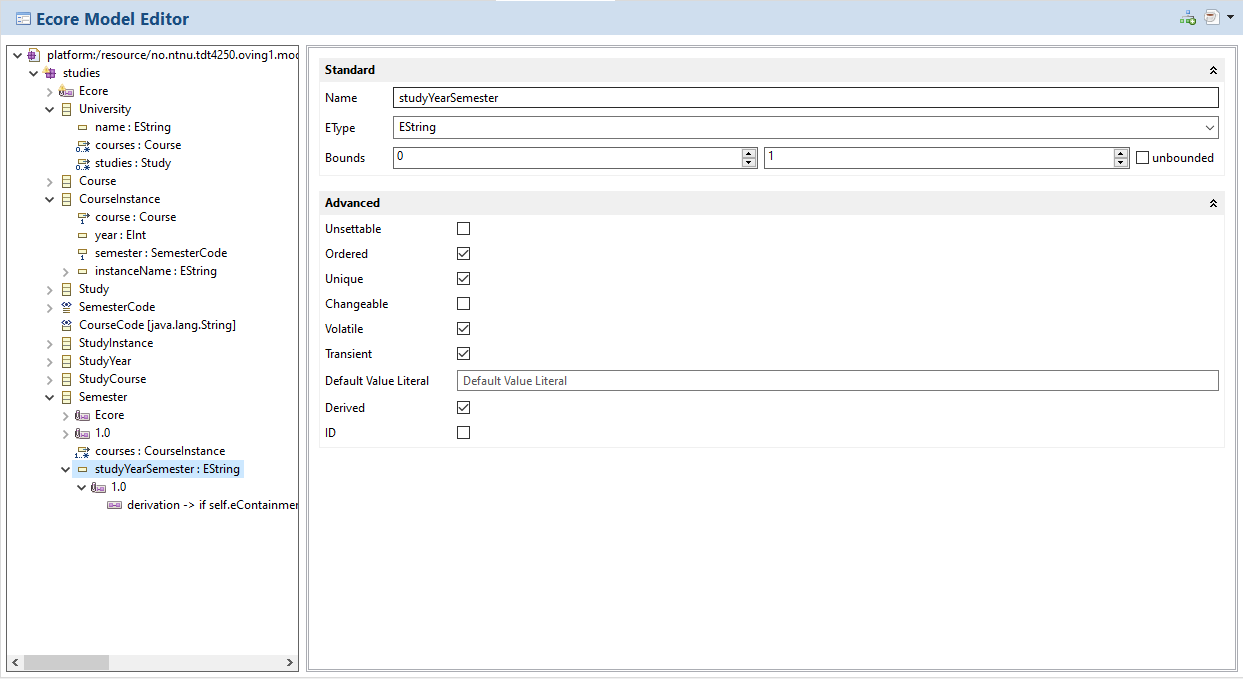
\includegraphics[width=\textwidth]{figures/pre-project/ecore-eclipse-emf-forms-model-editor.png}
  \caption[EMF Forms Ecore Editor]{A screenshot of a model in the EMF Forms based Ecore Editor.}\label{fig:emf-forms-ecore-editor}
\end{figure}

\iffalse{} 
{
%Skip diagrams for now. Tree editors are more important.

  \subsection{Ecore Tools diagrammatical editor}\label{sec:ecore-tools-editor}
  
  The \textit{Ecore Tools} editor presents \gls{Ecore} as class diagrams, similar to \gls{UML} Class Diagrams.
  
  \subsection{EMF.Cloud ecore-glsp diagrammatical editor}\label{sec:ecore-glsp-editor}
  %TODO
  
}
\fi


%* Eclipse EMF offers different Ecore editors. Tree-editor is important for developers, and diagrams are important in runtime and end-users.



\section{Introduction to Tree Structures}\label{sec:tree-structures}

\paragraph{Rationale}
Because the editors center around a tree structure, a clear understanding of trees is helpful.

\paragraph{Trees}
A \textit{tree} is a data structure.
The tree is composed of \textit{nodes}, and one node is designated as the \textit{root node} node or \textit{tree root}.
Each node can have zero or more \textit{children} nodes, and one \textit{parent} node.
The root node does not have a parent.
When representing the tree as code, it is possible to omit either the parent or child relationship in a node, making the parent or child implicit.
The relationship can still be found, by \textit{traversing} the tree.
Traversing means to visit every node it the tree by following the parent or child relationships.


\paragraph{Visualizing trees}
There are many ways to present trees to humans.
Two common approaches are \textit{hierarchy} and \textit{diagram}.


In a hierarchy, the parent is presented as a row, and its children on separate rows below (see \cref{sfig:tree-visualized-hierarchy}).
The children are often indented as well, and possibly connected with dots or lines to the parent.


In a diagram, nodes are often displayed as a circle or box (see \cref{sfig:tree-visualized-diagram}).
The parent is displayed above its children, and the children are aligned on the same row.
The parent-child relationship is shown as a line or arrow, connecting the parent to the child.

\begin{figure}[htbp]
    \centering
    \begin{subfigure}[b]{.45\textwidth}
        \centering
        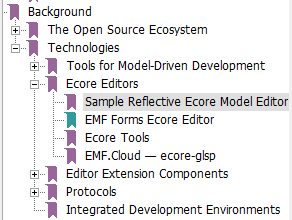
\includegraphics[width=\textwidth]{figures/tree-hierarchy.png}
        \caption{A tree visualized as a hierarchy. The top node is the root.}\label{sfig:tree-visualized-hierarchy}
    \end{subfigure}
    \hfill
    \begin{subfigure}[b]{.45\textwidth}
        \centering
        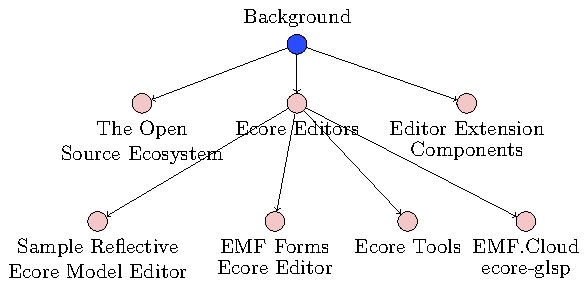
\includegraphics[width=\textwidth]{figures/tree-diagram.pdf}
        \caption{A tree visualized as a diagram. The blue node at the top is the root.}\label{sfig:tree-visualized-diagram}
    \end{subfigure}
    \caption{A tree visualized as a hierarchy and diagram. The labels are section titles of \cite{rekstadModelingEnvironmentCloud2020}, as an example.}\label{fig:tree-visualized}
\end{figure}

\paragraph{Nodes}
The tree is more useful when the nodes have properties.
The minimum property is children or parent.
But a useful property is a name, label or id, with regards to presenting the tree to a human.
There may be properties on the relationships between a node and its children, but these may be hard to present visually in hierarchy-type visualizations.
For a diagram type visualization, the properties may be presented as labels on the edge.

\paragraph{Mapping to trees}
A data structure can be mapped to a tree if it has separate objects with a containment or aggregation relationship.
There can be different ways to map to a tree, depending on what properties are used (or not used).
The labels can also come from various object properties, be derived from them or combine multiple properties into one label.



\section{Master-Detail Tree Editor}\label{sec:master-detail}

\paragraph{Rationale}
The tree editors use a layout pattern called \textit{master-detail}.

\paragraph{Description}
As the name \textit{Tree Editor} implies, they are used to edit a tree.
There are mainly two different things that can be edited: the parent-child relationships and the node's properties.
The user interfaces for the tree editors in \cref{sec:emf-editors} use a pattern called \textit{master-detail}.
This means the user interface is composed of two parts: a \textit{master view} and a \textit{detail view}.
% TODO: add a figure of master-detail overlayed on an editor?


\paragraph{Master view}
The tree structure is shown as a hierarchy in the master view.
It is common for the master view to be positioned to the left of a detail view, or above it.
The user interacts with the master view to add, remove and select nodes.
Adding a new child to a parent is done here.


\paragraph{Detail view}
When a node is selected, its properties are displayed in the detail view.
It is common for the detail view to be positioned to the right of a master view, or below it.
The detail view is usually a \textit{input form} or tabular (rows and cells) structure.
The user usually enters text, numbers, ticks checkboxes and opens selection dialogues from the detail view.


\section{The Eclipse Reflective Ecore Editor}

* Reflective Ecore Editor, its architecture, Commands in .Edit, works on any model.
% TODO: remove? DUplicate of prev. section?

\section{An Overview of EMF:\ Ecore Metamodel, XMI Serialization and GenModel for Code Generation}\label{sec:emf-metamodel}
%TODO

\paragraph{Rationale}
%TODO

\paragraph{\acrlong{EMF}}
%TODO
% eclipse editor plugins, language, codegen, ocl, serialization format

\paragraph{Ecore metamodel}
%TODO
% Class, package, attribute, reference

\paragraph{\Acrshort{XMI} serialization}
%TODO
% serialization, standardized EMOF, default for ecore, XML,

\paragraph{Ecore java \acrshort{API}}
%TODO
% EPackage registration, instance, factory, EList, EditingDomain, ItemProvider, Resource and ResourceSet

\paragraph{GenModel code generation}
%TODO
% Template based, configuration options, model + .edit + .editor output

\paragraph{Custom code}
%TODO
% editing genmodel code. @generated NOT annotation


* Ecore metamodel, EMF, XMI, genmodel. Adaptation of editors to special cases like Ecore model and Genmodel.

\section{Visual Studio Code's Custom Editor API}\label{sec:vscode-custom-editor}
%TODO
* VSCode Custom Editor API enables any type of graphical editor to be made, not just text.

\section{Language Server Protocol Architecture}\label{sec:lsp}
%TODO
* LSP from VSCode solves language-to-editor m*n combinations. There is already a need to move EMF from Eclipse to VSCode, it might need to move to IntelliJ etc. in the future.
* Monaco general frontend. Also Eclipse uses LSP with JDT? IntelliJ??

\section{\Gls{cloud} and \gls{Gitpod}}
%TODO

\section{\acrlong{EMF} in the \Gls{cloud}}
%TODO
* Recent development, EMF.Cloud Model Server, EMF.Cloud EMFJson, GLSP, GLSP Ecore Editor, GLSP Coffee Editor.

\section{Pre-project Results}

\subsection{Research Questions}

The pre-project started by asking the following research question:
\begin{quote}
\textit{How can we modernize Model-Driven Development Frameworks to appeal to
the next generation of software developers, using recent developments in cloud
IDEs?}~\cite[p.~3]{rekstadModelingEnvironmentCloud2020}
\end{quote}

After answering this question, the pre-project narrowed down to the following research question:

\begin{quote}
\textit{How can we design an Ecore master-detail tree editor that works in both VSCode and Theia, while reusing existing tools for Ecore such as codegen and validation?}~\cite[p.~24]{rekstadModelingEnvironmentCloud2020}
\end{quote}

A set of five related sub-questions were also posed, and subsequently answered.
These questions set the context for a solution, and the stakeholders, constraints and requirements that would be needed.
The following subsections (\ref{subsec:stakeholders} to \ref{subsec:pre-project-protocol}) will present the results of the pre-project that are the basis of work done in this thesis.

\subsection{Stakeholders}\label{subsec:stakeholders}

A stakeholder is someone affected by or interested in the solution.
It can be an organization or people~\cite[p.~52]{bassSoftwareArchitecturePractice2013}.
The pre-project identified the key stakeholders in \cite[p.~3]{rekstadModelingEnvironmentCloud2020} to be:

%TODO use a table?
\begin{itemize}
  \item Kristian Rekstad (author). Goal: increase adoption of \acrshort{MDD} by students and industry. Has to design and develop the initial solution.
  \item Hallvard Trætteberg (supervisor). Goal: teach students the concepts of \acrshort{MDD} in \gls{TDT4250}. Wants to use \gls{Gitpod} and \acrshort{EMF} for student assignments.
  \item Teachers/Lecturers that use \acrshort{EMF}. Goal: teach students. Have to present the tree editor, use it and support students that ask for help.
  \item Students. Goal: learn useful technologies and pass courses like \gls{TDT4250} to get a grade. Will have to use \acrshort{EMF} if they study Computer Science with the ``Software Engineering'' specialization at \acrshort{NTNU}.
  \item Industry professional using \acrshort{EMF} to do \acrshort{MDD}. Goal: develop software for a business/client. May want to use \acrshort{EMF} without using \gls{Eclipse}, for personal reasons or organization policy.
  \item Eclipse Foundation. Goal: foster a community of developers and provide open source software. The maintainers of \acrshort{EMF}.
  \item Eclipse ecosystem developers. Goal: contribute to Eclipse Foundation projects. May possibly have to maintain and further develop this (or a derivative) solution if this project succeeds and they embrace it.
  \item Developers of third party \gls{VSCode} extensions that use tree editors. Goal: provide a high quality editor for their specific problem domain. Could use the architecture, protocol and frontends of this solution, if this solution is high enough quality, architected to be reusable and partially independent of \acrshort{EMF}, and reuse will reduce their design and/or development time.
\end{itemize}

\subsection{Software Requirements}

\paragraph{Requirement engineering approach}
The pre-project tried to establish the software requirements for a tree editor.
A literature review failed to find related works that listed the requirements for a tree editor.
The literature review also failed to find related works for modeling in the cloud with the purpose of creating \gls{Ecore} models.
The related works either \textit{deployed} \gls{Ecore} models to the cloud, were textual editors, or did not use \gls{Ecore}~\cite[p.~3]{rekstadModelingEnvironmentCloud2020}.


Without literature to suggest requirements, and without users to test on (except the author and supervisor), the best option was to analyze the existing tree editors in \gls{Eclipse}.
Common modeling tasks were performed (see \cref{par:tdt4250-confluence}), and detected functionality was recorded.
The result gave an initial list of functional requirements, but not a complete one.
However, by following an agile approach instead of waterfall, this list does not need to be complete\footnote{Agile values working software over extensive documentation, thus spending time on creating a working solution is better than a ``worthless'' list of everything a solution \textit{could have done}.}.
More requirements will emerge naturally as work progresses.
Still, having a good overview of the requirements is needed to correctly decide a software architecture, because of ``architecturally significant requirements'' that affect the architecture~\cite[p.~291]{bassSoftwareArchitecturePractice2013}.

\paragraph{Constraints}
A constraint is a restriction on the available choices for a solution~\cite[p.~7]{wiegersSoftwareRequirements2013}.
The most important constraint discovered was that the tree editor must be a \gls{VSCode} extension.
There is an alternative extension mechanism for \gls{Theia}, which was deemed incompatible with \gls{Gitpod}%
\footnote{Gitpod can use Theia as its editor frontend, but the user is not allowed to recompile and upload a new version of Theia. The alternative extension mechanism, \textit{Theia Extensions} needs a full recompilation of Theia~\cite[p.~38]{rekstadModelingEnvironmentCloud2020}. However, VSCode extensions can be installed during runtime, also in Theia in Gitpod.}%
~\cite[p.~38]{rekstadModelingEnvironmentCloud2020}.


\paragraph{Functional requirements}
A functional requirement specifies \textit{what} a solution must do, such as supported features~\cite[p.~7]{wiegersSoftwareRequirements2013}.
The pre-project identified several functional requirements for a tree editor in the cloud.
The full list of functional requirements, with id, requirement and description can be found in \cref{app:functional-requirements}.
The list can be summarized as follows:

\begin{itemize}
  \item Provide a master-detail tree editor in VSCode and Theia (Gitpod) by using an extension mechanism of the \gls{IDE}.
  \item The tree editor must show nodes with labels and icons as a hierarchy.
  \item Allow selecting a node in the tree editor by clicking it.
  \item Provide a property sheet for the selected node in the tree editor.
  \item Provide an action bar with actions that can be dynamically specified by a backend server.
  \item Child nodes can be hidden or shown in the tree by a user.
  \item The tree editor and property sheet must update when the underlying model changes in the server.
  \item The action bar shows appropriate actions based on the selected node.
  \item The tree editor must allow creation of new nodes.
  \item The tree editor must allow deleting nodes.
\end{itemize}

Some more important requirements were implicit, and not defined in the list.
This was not intentional, and an evidence to the list's non-completeness.
Some of the implicit requirements are explicitly defined as follows:

\begin{itemize}
  \item The editor must handle \gls{Ecore} models.
  \item The editor must handle model instances from \acrshort{XMI} files.
  \item The tree structure must be based on containment properties in the \gls{Ecore} model.
  \item The editor must provide a command in the \acrshort{IDE} to create a new \gls{Ecore} file with the minimum \acrshort{XMI} needed for a valid empty model.
  \item Tree nodes can be moved to new parents by drag-and-drop by the user.
  \item The drag-and-drop can not let the user drop a node on a parent that cannot contain the node as a child. 
  \item Saving a model will serialize it as \acrshort{XMI} to a file on disk.
  \item An action in the action bar must be added to run \textit{model validation}.
  \item An action in the action bar must be added to run \textit{code generation}.
  \item The editor shall show multiple tree roots when there are related model files. Opening a \gls{Ecore} file shall also show any genmodel file. A model instance shall also include a root for the \gls{Ecore} model in the same editor.
  \item A user can open more than one unique \gls{Ecore} model at the same time, in separate ``tabs'' in the editor.
  \item Any modification to the model must support undo and redo.
\end{itemize}


\paragraph{Non-functional requirements}
A non-functional requirement specifies characteristics or properties of the solution~\cite[p.~7]{wiegersSoftwareRequirements2013}.
Most of the non-functional requirements are grounded in empirical evidence like what the Eclipse ecosystem and web development ecosystems are currently doing.
A non-formal list of the non-functional requirements is as follows:

\begin{itemize}
  \item Compatibility with a code editor in \gls{Gitpod}.
  \item Use a permissive \gls{open source} license.
  \item Avoid software dependencies that are closed-source or use restrictive licenses.
  \item Use a distributed architecture with components reuseable in other \acrshortpl{IDE}, inspired by architectures already in use by similar solutions~\cite[p.~24]{rekstadModelingEnvironmentCloud2020}.
  \item Configurability of user-facing options. Choices of colors, fonts, file system paths and similar should be possible to change~\cite[p.~24]{rekstadModelingEnvironmentCloud2020}.
  \item Configurability of mapping of \gls{Ecore} models to trees. Which containment references to use as children, and custom logic for labels should be user-specifiable~\cite[p.~24]{rekstadModelingEnvironmentCloud2020}.
  \item Localize the user interface in English.
  \item Flexibility and extensibility in the protocol to the server, allowing custom messages~\cite[p.~24]{rekstadModelingEnvironmentCloud2020}.
\end{itemize}


\subsection{Architecture and Protocol for a Solution}\label{subsec:pre-project-protocol}

A specific software architecture was proposed.
It had a goal to solve the requirements for: software reuse, \gls{Theia} and \gls{VSCode} compatibility, tree hierarchy editing, and a solution that could be transferrable to other tree domains and editors.
Additionally, the protocol would try to stay close to related solutions, as they are empirically tested and familiar to developers in the Eclipse ecosystem.
By creating prototypes, major ``blockers'' or risk factors of the proposed architecture was tested and proven non-problematic~\cite[p.~38-46]{rekstadModelingEnvironmentCloud2020}.


\subsubsection{Architecture}

The tree editor shall be a \gls{VSCode} extension, and use the available \acrlongpl{API} for \gls{VSCode} extensions.
No dependencies to \gls{Theia} shall be introduced.
To view the tree structure as a hierarchy, the \textit{Custom Editor API} in \gls{VSCode} must be used (see \cref{sec:vscode-custom-editor}).
A custom editor can present the editor inside \gls{VSCode} as a \textit{WebView}, meaning a custom webpage free to render anything, isolated from the rest of \gls{VSCode}.


\paragraph{Components}
The editor thus comprises 4 components: the tree editor WebView (``\textbf{editor frontend}''), the \gls{VSCode} extension integration (``\textbf{extension}''), a \textit{Tree Language Server} (``\textbf{TLS}'') and the \textit{EMF.Cloud ModelServer} (``\textbf{ModelServer}'')~\cite[p.~48,49]{rekstadModelingEnvironmentCloud2020}.
An illustration is shown in \cref{fig:pre-project-tree-editor-architecture}

\begin{figure}[htbp]
  \centering
  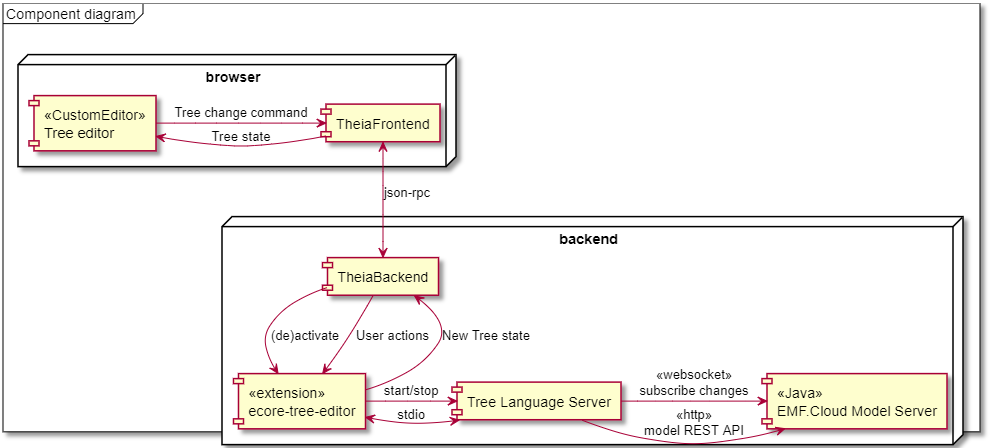
\includegraphics[width=\textwidth]{figures/pre-project/tree-editor-component-diagram.png}
  \caption[Tree Editor Architecture]{A suggested architecture for a tree editor. Copied from Figure 5.15~\cite[p.~49]{rekstadModelingEnvironmentCloud2020}. The diagram is based on \gls{Theia}, and the \gls{JSON-RPC} between TheiaFrontend and TheiaBackend happens behind the scenes, and is therefore not relevant to discuss.}\label{fig:pre-project-tree-editor-architecture}
\end{figure}


\paragraph{Editor frontend}
The editor frontend must be a web application that renders the tree as HTML, and provides interactivity with javascript. 
It communicates to the extension using \textit{messages} containing \gls{JSON}\footnote{This is a constraint imposed by the WebView API in VSCode.}.
The editor frontend will send messages that are \textit{commands} with the changes or actions a user triggered.
The extension will send messages with the new tree state to be shown.

\paragraph{Extension}
The extension is the main artifact which a user will install into \gls{VSCode} or \gls{Theia}.
This must be implemented with the \gls{TypeScript} language or javascript.
The extension will bundle the compiled code for the editor frontend, TLS and ModelServer inside it.
The extension is responsible for integrating with the \gls{IDE}, so that model files are opened in the custom editor, and handles commands triggered by the user in the \gls{IDE} (such as actions to create a new file, or saving a model).
The extension will start and stop the TLS process, and communicate over a \gls{JSON-RPC} protocol or \gls{REST} plus \gls{WebSocket}.
The extension and TLS can either use TCP sockets or standard in/out as the transport.

\paragraph{TLS}
A Tree Language Server (TLS) will contain specific knowledge about \gls{Ecore} and \acrshort{EMF}.
The choice of programming language is unconstrained.
The main purpose of the TLS is informing the extension of tree state, provide configuration for the tree editor and extension, and receive commands to modify models.
The TLS must be able to communicate using the same protocol as the extension (\gls{JSON-RPC} or \gls{REST} and \gls{WebSocket}), and either do so over standard in/out, or listen to incoming TCP sockets.
The TLS will perform commands to modify \acrshort{EMF} models by using as much re-use of existing code and frameworks as possible.
The TLS will start the ModelServer and communicate with it to read and modify models.
The ModelServer is a main part in the strategy to re-use existing code.

\paragraph{ModelServer}
This is a component already made by EclipseSource in java.
The ModelServer exposes \gls{REST} endpoints for working with \acrshort{EMF} models, such as listing models, reading models, and changing models with the EMF Commands framework.
Changes to a model are exposed as \gls{WebSocket} endpoints which can be ``subscribed'' to.


\subsubsection{Protocol}
The communication between the extension and the TLS should follow a defined protocol.
The protocol will contain the data structures and message formats to send, the serialization standard to use for messages, and define any required order for messages.


\paragraph{Base protcol}
The pre-project did not progress far enough to formally define this protocol, and did not implement it (or an alternative) either.
However, it specified a starting point and some rules.
The protocol should draw inspiration from the \acrlong{LSP}, and use the ``Base Protocol'' defined in \acrshort{LSP}.
The Base Protocol has two parts: a HTTP header section, and a \gls{JSON-RPC} content section~\cite[p.~17,18]{rekstadModelingEnvironmentCloud2020}.
The header section will at minimum include a \textit{Content-Length} field, specifying the number of symbols in the content section.
The content section will specify the remote procedures to be called, and the contain responses with data, such as tree structures, success or failure status, and errors.



\paragraph{Data structures}
This protocol can use the data structures to contain generic tree structures, proposed in Code listing 5.3 in \cite[p.~43,44]{rekstadModelingEnvironmentCloud2020}. %TODO: add code listing to appendix?
The protocol can not contain any specific references to \acrshort{EMF}, except as values in the generic data structures.
The central properties in the tree strucure was \textit{name}, \textit{type}, \textit{id} and \textit{children}.
The \textit{type} would for \gls{Ecore} be one of for example: \text{EClass}, \textit{EPackage}, \textit{EReference} and so on.


The action bar should be populated based on a ``action schema'' data structure (Code listing 5.4 and 5.5 in \cite[p.~45]{rekstadModelingEnvironmentCloud2020}), passed from the TLS to the extension in the protocol.


The hierarchy should be constrained by using a ``hierarchy schema'' (Code listing 5.6 in \cite[p.~45]{rekstadModelingEnvironmentCloud2020}).
This would whitelist the allowed children for a node based on the \textit{type} property.
This would be passed from the TLS to the extension.



\section{Open Source Software Project Management and Project Viability}

* What can make this Open Source software project viable and worth pursuing further? Anecdotal and empirical evidence, not research.
  * This project needs to live on after the delivery of the Thesis.
  * Correct open source licenses, and "licence hygience" wrt. copy-pasting. Eclipse Foundation do thorough licence reviews.
  * Use of programming languages accepted by the developer community.
  * Use of automated build systems accepted by the developer community.
  * Testable code to reduce legacy and maintenance burden.
  * Human readable, clean code. Correct use of Design Patterns. Clean separation of concerns.
  * Use of commonly used and recognized dependencies/libraries/frameworks/tools.
  * CI/CD.
  * Good developer documentation. Architecture diagrams. Informative Readme-files with pictures of the running software. Instructions for developer environment setup.
  * Google Design Documents (?). Not too common in this ecosystem, but valuable inside Google. Complements the readme.
  * Publicly available bug/issue tracker and roadmap.
  * Release management. Semantic versioning. Changelogs. More useful for end-users or those using this as a library/dependency.
  * Specific to Eclipse Foundation, is the "Eclipse Foundation Project Handbook" (https://www.eclipse.org/projects/handbook/) and its checklist.
  * Measures to reduce new-developer onboarding and friction.

\chapter{Method}\label{chap:method}

The method used will try to achieve the project objectives with correct results, and avoid or lower risks for project failure.

\paragraph{Pre-project}
The pre-project that came before this master's thesis, in \cite{rekstadModelingEnvironmentCloud2020}, is regarded as a part of the methodology.
It did the initial steps of problem identification, building, and prototyping a solution.

\paragraph{Software project}
Alongside this thesis, \textbf{a software project} will be created, which is developed by the author as part of the method.
A substantial amount of time is dedicated to this project.

\paragraph{General failure criteria}
The project is a failure if the results are invalid, or cannot be realized into a real solution, or are so low quality that the project does not receive further development.
The project is also a failure if it does not provide any value for its stakeholders.

\paragraph{Method overview}
The following sections describe the key elements to the method.
There is an overarching approach, called Design Science Research.
It has 6 phases, from problem identification, to development, to evaluation and communication.
There is no methodology given by Design Science Research for executing the development phase.
Therefore, a method for this phase must be crafted from experience and existing practice.
The development phase consists of requirements engineering methods, and software development methods.


\section{Design Science Research}
%* Design Science. Build and evaluate value. Contribute to knowledge base. Is this software we need?


Design Science Research in information systems is a methodology for creating new knowledge by designing, building and evaluating software \glspl{artifact}.
It may not be as widely known as ``the scientific method'' is, and is therefore explained in more detail.

\paragraph{Design}
\textit{Design} in information systems is an iterative process and a resulting software artifact. A software artifact is to be built to solve problems for humans, and evaluated to prove it solves the problems~\cite[p.~2]{alanhevnerDesignResearchInformation2010}.


\paragraph{Research}
\textit{Research} is an activity that adds new knowledge and understanding about something.
Research should be systematical and use data to answer questions, solve problems and provide understanding~\cite[p.~2,3]{alanhevnerDesignResearchInformation2010}.

\paragraph{Design Science Research}
\textit{Design Science Research} is an approach to research where knowledge is created by design.
It is defined by \textcite[p.~5]{alanhevnerDesignResearchInformation2010} as follows:

\begin{quote}
  \textit{``Design science research is a research paradigm in which a designer answers questions relevant to human problems via the creation of innovative artifacts, thereby contributing new knowledge to the body of scientific evidence.
  The designed artifacts are both useful and fundamental in understanding that problem.''}
\end{quote}

The end goal of a Design Science Research project is to create information technology \glspl{artifact}, that improve exiting solutions or solve a problem for the first time~\cite[p.~6]{alanhevnerDesignResearchInformation2010}.
A similar methodology may also be known under the name \textit{Design and Creation}, as presented by \textcite[p.~108]{oatesResearchingInformationSystems2006}.
According to \textcite{alanhevnerDesignResearchInformation2010}, the artifacts are generally classified as \textit{constructs}, \textit{models}, \textit{methods}, \textit{instantiations} or \textit{better design theories}%
\label{par:artifact-classes}%
\footnote{This thesis aims to produce an instantiation: an implemented or prototype system. The thesis also seeks to advance on \textit{better design theories}, with regards to software architecture and protocol design.}.
A very important aspect of Design Science Research is \textit{evaluation} of the artifact.
The evaluation is the process that uncovers new knowledge, and separates the process from routine design~\cite[p.~7]{alanhevnerDesignResearchInformation2010}.
There are many aspects that could be evaluated, but the aspects that \textit{should} be evaluated are those that are related to the reason for creating the artifact in the first place; the aspects related to the research objectives~\cite[p.~115]{oatesResearchingInformationSystems2006}.


% TODO

\subsection{The General Design Cycle }

\paragraph{Design Cycle}
Problem solving by design can follow a general design cycle.
This is a circular and iterative process.
The reasoning that occurs in a design cycle, and the knowledge generated during a cycle, is illustrated in \cref{fig:dsrpm}~\cite[p.~26]{alanhevnerDesignResearchInformation2010}.

\begin{figure}[htbp]  % order of priority: h here, t top, b bottom, p page
  \centering
  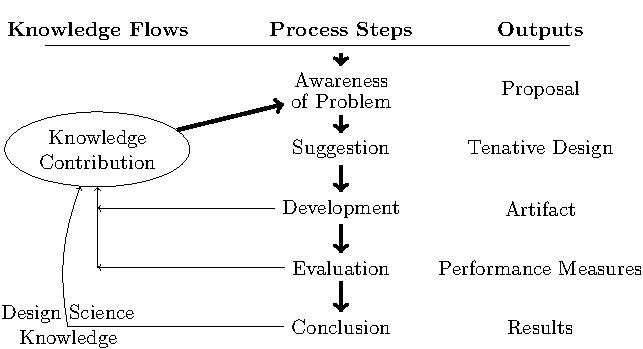
\includegraphics[width=\textwidth]{figures/dsrm-flow.pdf}
  \caption[Design Science Research Process Model]{\textbf{Design Science Research Process Model}. The general process followed by Design Science Research. Design begins with awareness of a problem, and progresses through a suggestion for a solution, to development, evaluation and a conclusion.
  The stages produce different outputs, shown in the right column.
  After the conclusion, new knowledge is contributed.
  There is also knowledge produced by development and evaluation, nicknamed ``circumscription''.
  This knowledge is fed back into a new round of suggestion~\cite[p.~11-13]{vijayvaishnaviDesignScienceResearch2019}.
  (Adopted from Figure 3 in \textcite[p.~11]{vijayvaishnaviDesignScienceResearch2019})}\label{fig:dsrpm}
\end{figure}


\paragraph{Awareness of Problem}
The process begins by becoming aware of a problem or opportunities, in the context of humans or an organization.
A proposal for what could be solved is made explicit.


\paragraph{Suggestion}
Then, a suggestion phase begins, where existing knowledge and theories are applied, as well as creativity, to create a tentative design that fits the proposal.
This design could be flawed or incorrect, which is why it is important to realize the design, to detect issues.


\paragraph{Development}
The development phase will build a solution or prototype, aiming to fulfill the suggested design.
This phase will uncover problems, inconsistencies, new learning about the problem, and other related knowledge.
That knowledge is useful for creating a new and improved design.
The quality of the \textit{implementation} of the artifact does not need to be novel, as it is the \textit{design} which is interesting~\cite[p.~12]{vijayvaishnaviDesignScienceResearch2019}.


\paragraph{Evaluation}
After an artifact is created, the evaluation phase will measure the artifact.
The measurements originate from the initial proposal, which holds the criteria for success.
This phase may also discover new knowledge, which can be used later to create a new and improved design~\cite[p.~13]{vijayvaishnaviDesignScienceResearch2019}.


\paragraph{Conclusion}
Finally, the conclusion phase will consolidate the results.
The knowledge gained from the results will either be ``firm'' or ``loose ends''.
\Textcite[p.~13]{vijayvaishnaviDesignScienceResearch2019} describes this as the following:

\begin{quote}
``\textit{Not only are the results of the effort consolidated and ``written up'' at this phase, but the knowledge gained in the effort is frequently categorized as either ``firm'' --- facts that have been learned and can be repeatedly applied or behavior that can be repeatedly invoked --- or as ``loose ends'' --- anomalous behavior that defies explanation and may well serve as the subject of further research.}''
\end{quote}


\subsection{Methodology}

Based on the understanding of design science research, and the steps of a design science research process (\cref{fig:dsrpm}), a six step Design Science Research Methodology has been made by \textcite[p.~28-30]{alanhevnerDesignResearchInformation2010}.
This methodology forms the skeleton of this thesis.
The six steps of the methodology are the following:

\begin{enumerate}
  \item \textit{Problem identification and motivation.}
  \item \textit{Define the objectives for a solution.}
  \item \textit{Design and development.}
  \item \textit{Demonstration.}
  \item \textit{Evaluation.}
  \item \textit{Communication.}
\end{enumerate}


\paragraph{1. Problem identification and motivation}
The specific research problem must be defined.
The definition is used to develop the artifact which solves the problem.
The value of a solution to the problem should be justified as well.
If the value of the solution is justified, it can motivate the researcher and the thesis' audience to pursue the solution and accept the results~\cite[p.~28,29]{alanhevnerDesignResearchInformation2010}.

\paragraph{2. Define the objectives for a solution}
The objectives should be inferred from the problem definition, and the author's knowledge of what is possible and feasible.
The objectives can be how much better a new solution should be (quantitative), or a description of how a new artifact would solve problems that are currently unsolved (qualitative)~\cite[p.~29]{alanhevnerDesignResearchInformation2010}.

\paragraph{3. Design and development}
Create an artifact to solve the problem and fulfill the objectives.
The artifact can be one of the five classes listed in \cref{par:artifact-classes} (constructs, models etc.).
The desired functionality and architecture is determined, and the actual artifact is created~\cite[p.~29]{alanhevnerDesignResearchInformation2010}.


\paragraph{4. Demonstration}
The artifact is demonstrated, to solve instances of the identified problem.
This could be experiments, simulations, case studies etc.~\cite[p.~30]{alanhevnerDesignResearchInformation2010}.


\paragraph{5. Evaluation}
The artifact is observed and evaluated to measure how well it solves the identified problem.
This can be done by comparing the results of the demonstration to the  objectives of an ideal solution.
There are many different ways to evaluate an artifact, and the correct approach should be decided based on the nature of the identified problem.
After evaluation, the researcher can go back to step 3 to improve the design.
If there is not enough time, resources or a need to do so, the process moves to step 6 instead~\cite[p.~30]{alanhevnerDesignResearchInformation2010}.

\paragraph{6. Communication}
The process must be communicated to other researchers and relevant audiences.
This communication includes: the problem and its importance, the artifact and its utility, the rigor of the artifact design, and the effectiveness of the design~\cite[p.~30]{alanhevnerDesignResearchInformation2010}.%
\footnote{This thesis is a central part of this communication.}




\section{Requirements Engineering}


In Design Science Research, there is little guidance for how to execute the actual \textit{design and development} phase.
However, the software engineering field has many approaches and ideas for how to do this.


The design of the artifact starts by gathering requirements.
These specify the concrete behaviors of the artifact; both the behaviors required for achieving the research objectives in \cref{sec:research-objectives}, and those required for a highly useable and valuable solution.


The identified requirements are both part of the design, and influence the design.
Most requirements are formed from existing knowledge of the background theory.
They are also discovered as the solution is developed.
The following subsections \ref{subsec:req-stakeholder}-\ref{subsec:req-agile} describe the key inputs for the software requirement engineering process.


\subsection{Stakeholder Discussion}\label{subsec:req-stakeholder}

Discussion with stakeholders reveal many requirements, use cases and needs.
The two key types of stakeholders here are \acrshort{EMF} experts and \gls{TDT4250} students.
The supervisor, Hallvard Trætteberg, fills the role as both a \acrshort{EMF} expert and lecturer of \gls{TDT4250}.
The author, Kristian Rekstad, fills the role as a \gls{TDT4250} student.


Dialogue questions include ``What features are required to model with \acrshort{EMF}?'' and ``What features would you like to see in a new solution?'', as well as ``Which features are missing from the existing solutions?''.


The same questions can be asked both before realizing a solution, and underway as the response to prototypes and current progress of an unfinished solution.


\subsection{Requirements Extraction}

\paragraph{Based on existing editors}
The existing tree editors in \gls{Eclipse} already implement every feature needed to do \acrlong{MDD} with the \acrlong{EMF}.
Therefore, they are excellent sources of requirements.
Especially the Sample Reflective Ecore Editor and EMF Forms Ecore Editor. %TODO: cref sections


\paragraph{No official requirements lists}
The pre-study failed to find any related research detailing requirements for a tree editor~\cite[p.~3]{rekstadModelingEnvironmentCloud2020}.
No design documents or requirements specifications were found for the \gls{Ecore} editors in \gls{Eclipse} either.


\paragraph{Use cases and requirement detection}
Therefore, the approach became to extract the requirements from the \gls{Ecore} tree editors.
The extraction is done by following use cases of modeling, as described in \cref{par:tdt4250-methodology}.
When a new functional requirement is discovered through use, it is recorded in a list.


\paragraph{Shortcomings}
This approach will find many of the required and ``obvious'' requirements.
However, hidden functionality and expert level functionality is not guaranteed to be found.
The rationale is that this functionality is not needed (yet) anyways, as the goal is to fulfil the common use cases that students have when learning \acrshort{MDD}.


There is also a risk that the user which is recording the requirements fail to detect functionality.
Some functionality can be so obvious or ``second nature'' that the user is oblivious to it.
Such functionality \textit{should} become apparent later, however, when the solution is developed and tested.
Any big omissions will prevent the use cases from succeeding.


\subsection{Source Code Analysis of Similar Projects}

\paragraph{Open source editors}
Because the tree editors for \gls{Ecore} in \gls{Eclipse} are \gls{open source}, it is possible to read and analyze the source code.
Finding the main classes responsible for editor functionality, and analyzing their method names, initialization procedures and method calls, may expose requirements.
This approach may also detect some of the more hidden functionalities, and the more ``internal'' functional requirements.


\paragraph{Architecture and software re-use}
Another advantage is that the internal architecture and patterns are exposed, which can be used to influence the artifact design.
This may increase familiarity with the design for the Eclipse ecosystem, aiding the \gls{open source} goals of this project.
It also highlights the opportunities for software re-use, when familiar code, classes, interfaces, design patterns or software libraries are used.


\paragraph{Shortcomings}
Source code analysis is dependant on analyzing the correct source code files.
If they are not found, this will fail.
This also requires the source code to have some level of quality and readability to be useful for someone not already invested in that editor code base.
The software architecture and design patterns used will matter too, in case functionality is hidden, dispersed or not clearly visible from the source code.


\subsection{Use Cases and Prototyping}

Creating realistic use cases based on \cref{par:tdt4250-methodology}, and executing them with early versions or prototypes will detect missing requirements.
This is because a user will be blocked from progressing if a critical functionality is missing.
%For example here: copy-paste, keyboard shortcuts etc)


\subsection{Agile Requirements}\label{subsec:req-agile}

\paragraph{Agile}
Core values during this thesis' requirements engineering process come from \textit{Agile}.
Agile is a counterpart to the Waterfall process\footnote{In waterfall, software is designed, developed and tested in very separate stages. All the requirements are collected, before any design or development begins. An early mistake will not be discovered until the very end of the process. Changes to requirements require a restart of the project phases.}


\paragraph{Change over Plan}
It embraces the fact that requirements change during the design and development, and thus favors \textbf{responding to change} over following a plan~\cite{kentbeckManifestoAgileSoftware2001}.
Requirements will change as they are discovered, refined and better understood later on.


\paragraph{Software over Documentation}
Another key value is that Agile prefers \textbf{working software} over comprehensive documentation~\cite{kentbeckManifestoAgileSoftware2001}.
This means that a small, working software artifact is more valuable than a large, complete and consistent list of software requirements and design, without any working software to show for it.


\paragraph{Impact of agile on requirements engineering}
The result is that the method here will start by collecting \textit{some} requirements, by using the previously described inputs.
When there are enough requirements to sufficiently solve the known use cases, design and development can begin.
There is no goal to create a complete list at the start.
The requirements are also changed, and new ones added, during the design and development.


\section{Development Methodologies}


The case for software development is the same as with requirements engineering: Design Science Research has little guidance.
And again, the software engineering field has the answers.


The goal for the development methodology is to \textbf{create the right solution}, which solves the identified problem and fulfils the software requirements.
The methodology also aims to \textbf{avoid or reduce risks} for project failure, by tackling it as early as possible.
Research often deviates from routine design here, by going for the risks first instead of delaying or hiding them, as this may lead to new knowledge~\cite[p.~114]{oatesResearchingInformationSystems2006}.


Another goal for the development process is to create ``good'', high quality software, so the project can be accepted by the \gls{open source} developer ecosystem for further development and maintenance.
Bad code or a bad design may result in a full rewrite by the next interested developer, or the developer may try to contribute but find it hard and give up.


Development methodology will not follow one strict practice, but rather piece together many different practices and values, which have lead to good results in the author's past.


\subsection{Agile}

Development will follow agile values and principles, as described in \citetitle{kentbeckManifestoAgileSoftware2001}~\cite{kentbeckManifestoAgileSoftware2001} and \citetitle{PrinciplesAgileManifesto}~\cite{PrinciplesAgileManifesto}.
This means readjusting plans, rapid feedback from stakeholders, and software that works underway in development.

\paragraph{Agile development}
As there are many unknown factors in development, such as third party components and services to comply and integrate with, and unknown and hard to use \glspl{API}, the plans and designs may change.
As with software requirements, the data structures, algorithms and design in the software solution will have to change as the developer learns the systems and problem space better.
\textbf{Responding to change} will be valued more than following a plan here.
Also, \textbf{working software} is more valuable than extensive documentation, meaning that code comments, tests, design specifications and diagrams will be given less effort than code, particularly if done up-front before the code.
The alternative is that this documentation is made, but the code for it quickly proves itself impossible to make, or there is not enough time to implement it, leaving only useless documentation as the result.
This also ties in to \textbf{simplicity and maximizing work-not-done}.


Regular reflection will be used weekly or bi-weekly, to assess if the process can be more effective.
Sometimes tools and technologies may seem like a good fit for the development, but instead wastes more time than the developer productivity provided.
Retrospective analysis of the development progress will try to detect this, and then expose if bad approaches are used.
If so, these will be removed or replaced if possible.


Stakeholder involvement is important as well.
The development will have a stakeholder as the developer (the author), which knows how the artifact will be used.
Additionally, the supervisor will see a demo during development, to provide feedback and help prioritize the next steps.


\subsection{Iterative Development}

The software system will be developed iteratively.
This means the components will be implemented up to a threshold of functionality, and executed to evaluate the behavior.
The evaluation is not a formal and rigorous one, but rather informal and aims to quickly confirm if the software has the correct behavior.
Then the components are developed some more, in a loop until the project ends.


The components are also developed incrementally.
It also means a component will be worked on until it reaches \textit{some} functionality, and then the next component will be worked on until it is on par.
No component is developed to completion while the others are not started on.


\subsection{Lean and Minimum Viable Product}

Lean development is a set of principles inspired from Lean Manufacturing (for automobiles and such)~\cite{rachellelynnGuidingPrinciplesLean}.


\paragraph{Eliminate waste}
A core principle is to \textbf{eliminate waste}.
This is also seen in Agile, as maximizing work-not-done.
What Lean regards as waste is any work and output that does not have value.
This means avoiding: unnecessary code and functionality (things deemed ``could be nice to have''), unfinished work in progress (code and features not completed), defects and poor quality (do it well, do it once).


\paragraph{Build quality in}
Another principle is \textbf{building quality in}.
Important business logic should have automated unit tests (however not all code needs tests\footnote{A project with high uncertainty and changing requirements may find tests a hinder as they have to up updated all the time. This results in extra work and rework.})
Tedious and repetitive tasks should be automated, for example with scripts and tools.


\paragraph{Create knowledge}
A third principle is to \textbf{create knowledge}.
Code will have comments where needed\footnote{Not all comments are good comments. Code with side effects, strange design choices or hard to read implementation may need clarification by using comments.}.
Documentation will explain the software at a high level.


\paragraph{Deliver fast}
The last principle applied is to \textbf{deliver fast}.
While there are no students to use the aritfact now, the focus is still on creating a functioning solution as early as possible.
This is done by prioritizing the requirements in an order to get a \textit{minium viable product} (MVP).
This is a solution that is just barely useable.
The goal is to get it into the hands of users as quickly as possible, because this creates valuable feedback.

\subsection{Tracer Bullets}

\paragraph{Tracer bullets}
Using Tracer Bullets in code is a metaphor from \citetitle{huntPragmaticProgrammerJourneyman2000}~\cite{huntPragmaticProgrammerJourneyman2000}.
When using a machine gun, the operator does not precisely calculate where to shoot ahead of time.
Instead, tracer bullets are occasionally loaded into the gun, which glow up and give visual feedback to the operator as to where the bullets travel.


\paragraph{Tracer code}
The same idea applied to coding means that uncertainty and risk is not dealt with by heavy upfront planning.
A software solution likely has to interface with many unknown parts, adding risk for each one.
The developer creates ``tracer code'', which has the goal of quickly connecting all the components and parts of the system, without adding lots of functionality.
Stubs and empty code can be used so the code compiles, as long as all the actual components in the final design are integrated and running.
If any problems are discovered, then adjust and redesign as necessary~\cite{huntPragmaticProgrammerJourneyman2000}. 


The tracer code is real code, not a prototype.
Therefore, it should be made with proper quality.
It just lacks functionality.
With a working skeleton system, more functionality can be added on top.


\subsection{Domain-Driven Design}

Domain-driven design is an approach to domain modeling in software.
The goal is to create a domain model in software that uses the same language a domain expert uses, to create better, more evolvable and understandable code.
If the domain has for example ``trees'' and ``nodes'', the code will also use trees and nodes as names, making stakeholder discussion straight forward.
The code will accurately model the domain, increasing understanding and capturing the details of the business logic~\cite{evansDomaindrivenDesignTackling2004}.
The model is represented as normal, executable code.
There is no specific file representation, and no \acrshort{MDD} framework involved.
This is not a \acrshort{MDD} method --- it is a object oriented coding and naming method.


Another element from Domain-driven design is to use a layered software architecture.
The domain model is isolated from the rest of the code.
This makes it easy to see and reason about the behavior of the code, in terms of business logic~\cite[p.~69]{evansDomaindrivenDesignTackling2004}.
The alternative is that business logic is spread around the system, partially in the user interface components, persistance logic, and so on.
The layers makes every aspect of the program more cohesive and makes interpretation of the designs easier~\cite[p.~69]{evansDomaindrivenDesignTackling2004}.


Practically, the domain model will be in its own layer, and the user interface will be in its own layer.
The user interface will depend on the domain model.
The domain model will be unaware of any user interface.
An illustration is shown in \cref{fig:ddd-layered}.

\begin{figure}[htbp]  % order of priority: h here, t top, b bottom, p page
  \centering
  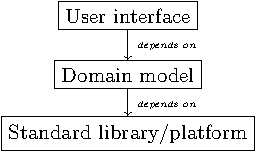
\includegraphics{figures/layered.pdf}
  \caption[Layered Architecture]{\textbf{Layered architecture}. The components above depends on the components below, but not vice versa.}\label{fig:ddd-layered}
\end{figure}


\subsection{Test-Driven Development}
%TODO

Test-driven development is about creating automated tests before writing the implementation~\cite[p.~105]{knibergScrumXPTrenches2015}.
It will be used sparingly, for cases where the behavior is complex and important to get right.
The developer will have to judge when it is needed, based on expected complexity, requirements and behavior for a unit of code.
This may be especially relevant for some business logic in the domain model.
Writing the tests first also creates a more testable design~\cite[p.~106]{knibergScrumXPTrenches2015}.


The benefit of automated tests is confidence in the code against bugs.
It also helps for when other developers join the project, as they can be confident about making changes without breaking existing code.
A goal is to have other contributors develop this project further, and therefore avoiding ``legacy code'' is a good thing.
The author of \citetitle{feathersWorkingEffectivelyLegacy2005} writes:

\begin{quotation}
``Legacy code is somebody else’s code. But in programmer-speak, the term means much more than that. 
[\ldots]


In the industry, \textit{legacy code} is often used as a slang term for difficult-to-change code that we don’t understand. 
[\ldots]


To me, \textit{legacy code} is simply code without tests. [\ldots]


Code without tests is bad code. It doesn’t matter how well written it is; it doesn’t matter how pretty or object-oriented or well-encapsulated it is. With tests, we can change the behavior of our code quickly and verifiably. Without them, we really don’t know if our code is getting better or worse.''


---~\textcite{feathersWorkingEffectivelyLegacy2005}
\end{quotation}


\subsection{Prototyping}

Prototyping will be used to create simple implementations when there is uncertainty of the design and big risks.
A prototype will create learning by coding in the real environment, and then prototype code is discarded afterwards.
A prototype can test feasibility and reveal good and bad sides of a design, quickly and cheaply.


The main bulk of prototyping has already been performed, as part of the pre-project in \cite{rekstadModelingEnvironmentCloud2020}.



\section{Evaluation}


This section will describe how the evaluations for the artifacts were made.
The evaluations try to test for value in the solution design, by comparing how well the artifacts solve the identified problem.

\subsection{Software Artifact}

The built artifact is evaluated according to the Design Science Research methodology in \cref{par:dsrm-demonstration}.

\paragraph{Assumptions}
The functionality of the original \gls{Eclipse} editors for \gls{Ecore} is assumed to be correct and useful for students.
The functionality is also required, in order to effectively use \acrshort{EMF} for \acrfull{MDD}.

\paragraph{Demonstration goal}
Therefore, a demonstration should show the presence of the original functionality from \gls{Eclipse} in the new artifact.
To do this, the artifact will be used to complete \textit{use cases}, based on the modeling approach used in \gls{TDT4250} (see \cref{par:tdt4250-methodology}).\\


Additionally, a goal is to not use the \gls{Eclipse}, and a goal is to perform the use cases in a \gls{cloud} based \gls{IDE}, in this instance \gls{Gitpod}.


\paragraph{Evaluation of demonstration}
The evaluation%
\footnote{The evaluation is classified as \textit{ex ante} and \textit{artificial}, for those familiar with the approach by \textcite{sonnenbergEvaluationsScienceArtificial2012} and \cite{venableComprehensiveFrameworkEvaluation2012}.} 
will be a list of tests with modeling actions from \cref{par:tdt4250-methodology}.
A test is successful if the tester (the author) can perform the action, and without using \gls{Eclipse} and also doing it in \gls{Gitpod}.


\subsection{Open Source Viability}

\paragraph{Evaluation goal}
A goal of this thesis is that the artifact's source code is developed further, by either master students, the Eclipse ecosystem, or other contributors with interest in \acrshort{EMF} or tree editors.
The strategy to solve this is by making the source code \gls{open source}.


Therefore, the source code will be evaluated to indicate how fit it is to be an \gls{open source} project.


\paragraph{Test criteria}
To test how fit the project is, a checklist is synthesized from online guides for open source projects.
The sources are highly reputable, such as the Eclipse Foundation, the GitHub community, and sites endorsed by these.
The criteria will check for presence of elements or properties of the project, and succeed if it is present.
A qualitative evaluation will proceed, to conclude the test results.


\chapter{Results}\label{chap:results}

This chapter will present the outcomes of the design and development phase.
First, the artifact is presented from a user's point of view, showcasing functionality with screenshots.
Then, the artifact's design will be presented from an architectural view, and the protocol will be presented last.\\

The results will also present the measures taken for making the \gls{open source} project viable, and something a developer community may want to develop and maintain further.\\

Evaluation of the results is presented later, in \cref{chap:evaluation}.

\section{Software Artifact: Tree Editor Extension for Ecore in Gitpod}

This is of interest for a stakeholder, and someone aiming to do further research on this design.

The output of the development phase is an artifact which is a \gls{VSCode} extension.
The artifact is a \texttt{.vsix} file, and can be installed in a \gls{Gitpod} workspace.
The following results are from \gls{Gitpod} using \gls{VSCode} as the editor frontend, not \gls{Theia}\footnote{VSCode is supposed to become the default for Gitpod in the future, instead of Theia~\cite{georgetsiolisMenuEntryGitpod2019}.}.
One way to install it\footnote{The ``best'' way is to publish the extension to OpenVSX, and search for it in the extensions panel.}, is to upload the \texttt{.vsix} file to the workspace, right clicking on it and selecting ``Install Extension VSIX''.
When installed in the \acrshort{IDE}, it is shown in the extensions panel as \textit{Ecore Tree-editor}, shown in \cref{fig:gitpod-ext-installed}.

\begin{figure}[H]  % order of priority: h here, t top, b bottom, p page
  \centering
  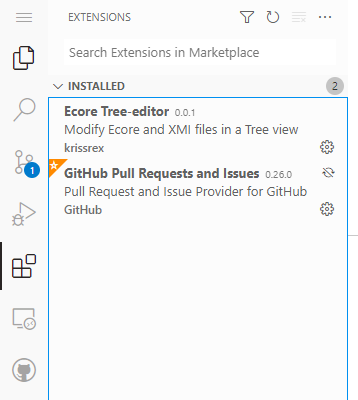
\includegraphics[width=0.6\textwidth]{figures/gitpod-vscode-extensions-installed.png}
  \caption[Tree Editor Extension installed in Gitpod]{The extension is installed as \textit{Ecore Tree-editor} in Gitpod with VSCode.}\label{fig:gitpod-ext-installed}
\end{figure}

\subsection{Custom Editor}

This extension adds a new Custom Editor, which is automatically opened when the user opens a \texttt{.ecore}, \texttt{.genmodel} or \texttt{.xmi} file.
The model file is loaded and transformed by the extension, and presented as a tree to the user.

\begin{figure}[H]  % order of priority: h here, t top, b bottom, p page
  \centering
  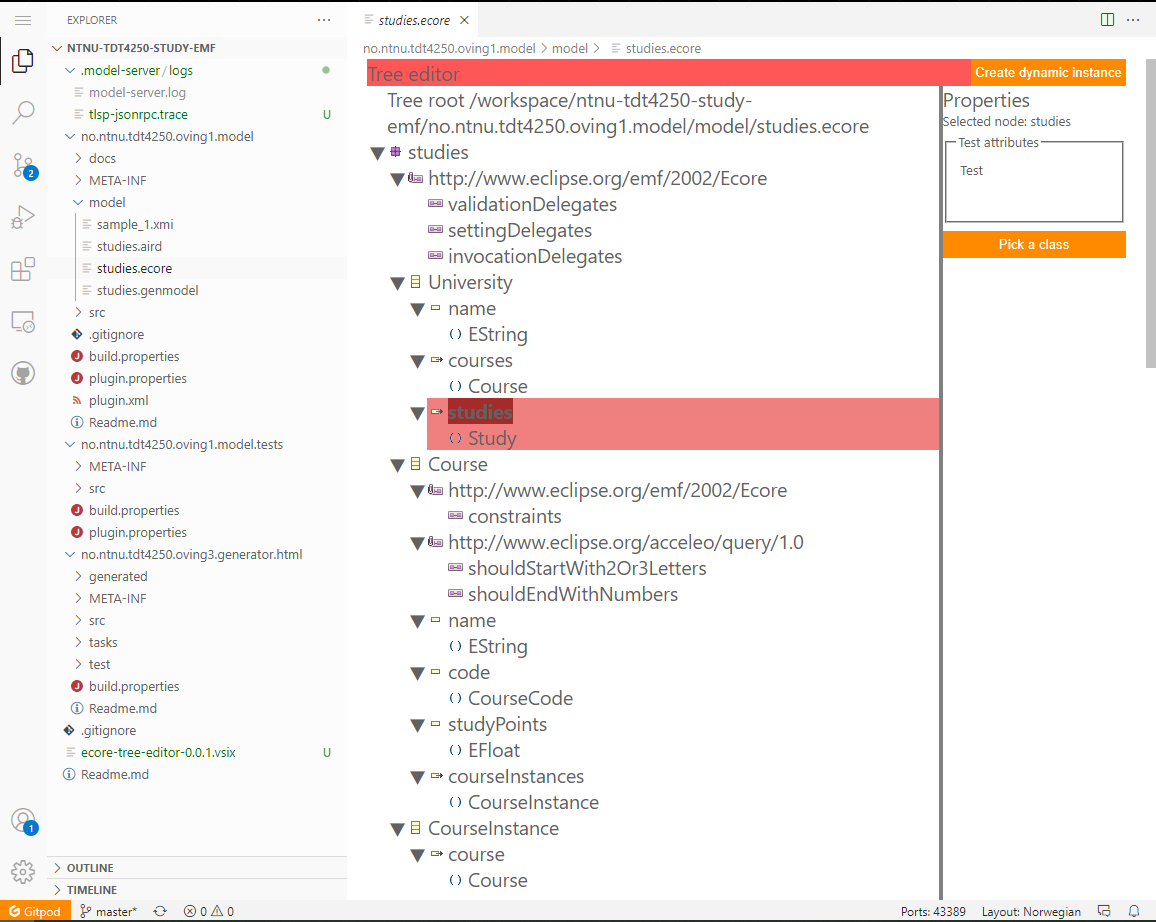
\includegraphics[width=\textwidth]{figures/gitpod-vscode-ecore-editor-studyemf.png}
  \caption[Tree Editor Extension showing studies.ecore]{The Tree Editor Extension has opened a Custom Editor for the \texttt{studies.ecore} file.}\label{fig:gitpod-ext-tree-ecore}
\end{figure}

\paragraph{Example model}
An \gls{Ecore} model made in \gls{TDT4250} in 2019 has been used as an example to demonstrate the artifact.
The \texttt{.ecore} file is opened in \cref{fig:gitpod-ext-tree-ecore}.
This figure shows three columns, from left to right: the default \gls{VSCode} file explorer, the custom editor's master layout (tree structure), and the custom editor's detail layout (properties sheet).

\paragraph{Action bar}
There is also a red action bar at the top, with an orange action button to create a new dynamic instance.
The action buttons shown will vary, depending on what the selected node is.
The orange color of the button is coming from the color theme of the \gls{VSCode} editor.
With a dark theme, this action button could be blue, for example.

\paragraph{Master layout}
The master layout can show multiple roots.
In this document,  single root is shown for the ``studies.ecore'' file.
The root node is a ``studies'' package, with children displayed below.
This node has a label, ``studies'', and a specific icon indicating it is a package --- the purple box with a cross.
The icons used are the same ones used in \gls{Eclipse} for the Sample Reflective Ecore Editor (see \cref{sec:sample-reflective-editor}), and depend on the type of node.

Clicking the black triangle next to a node will collapse it, hiding its children and rotating the triangle 90 degrees counter-clockwise.

Inside the master layout, a node is selected in dark red, with the label ``studies''.
Its child node ``Study'' is also highlighted, in a lighter red.
(Note that the colors of selected nodes were arbitrarily chosen during development, and could be changed to give more contrast with the node's label.)
A node can be selected by clicking on it, and holding \texttt{ctrl} will add to the selection, allowing multiple nodes to be selected.

Dragging a node in the hierarchy and dropping it on a node, should change this node's parent.
Right clicking a node will open a context menu, with the possible children nodes to add.
Dropping a node on an invalid parent will be prevented, by using a hierarchy schema, and indicated by changing the mouse cursor to a ``forbidden'' icon\footnote{Note that drag-and-drop and node creation are not currently implemented, only accounted for by the design, by using a hierarchy schema.}.


\paragraph{Detail layout}
The detail layout has a property sheet, currently showing a unfinished example form.
This layout should use the \textit{JSON-Forms} library to render properties, based on the node's properties and a \textit{UI schema} for that node type.


\subsection{IDE Commands}

The extension also provides Commands to \gls{VSCode}.
These are actions that can be invoked at any time.
The student can invoke them from the Command Palette\footnote{Press \texttt{F1}, or \texttt{ctrl + shift + P} (command on mac), or \texttt{Menu $\rightarrow$ View $\rightarrow$ Command palette}} by typing ``Ecore'' or another part of the command's name.
A screenshot is shown in \cref{fig:gitpod-ext-newmodel}, with a command to create a new model file.
This file will have the minimum \acrshort{XMI} contents required for a blank model.

\begin{figure}[H]  % order of priority: h here, t top, b bottom, p page
  \centering
  
\includegraphics[width=\textwidth]{figures/gitpod-vscode-newmodel.png}
  \caption[Tree Editor Extension Custom Commands]{The Tree Editor Extension adds custom commands to the Command Palette. One of them is shown here, named \textit{Ecore: New Model file\ldots}.}\label{fig:gitpod-ext-newmodel}
\end{figure}

\subsection{Genmodel and Model Instance}

The editor can open a \texttt{.genmodel} file or a \texttt{.xmi} model instance file as well.
The GenModel is shown in \cref{fig:gitpod-ext-genmodel}, and the dynamic instance in \cref{fig:gitpod-ext-dynamic}.
This will show two roots in the editor, as the original \texttt{.ecore} model is related to the opened file.
One root is the GenModel or model instance, and the other root is the study model.

The GenModel editor is not specialized, so it renders the tree as any other \gls{Ecore} model.

\begin{figure}[H]  % order of priority: h here, t top, b bottom, p page
  \centering
  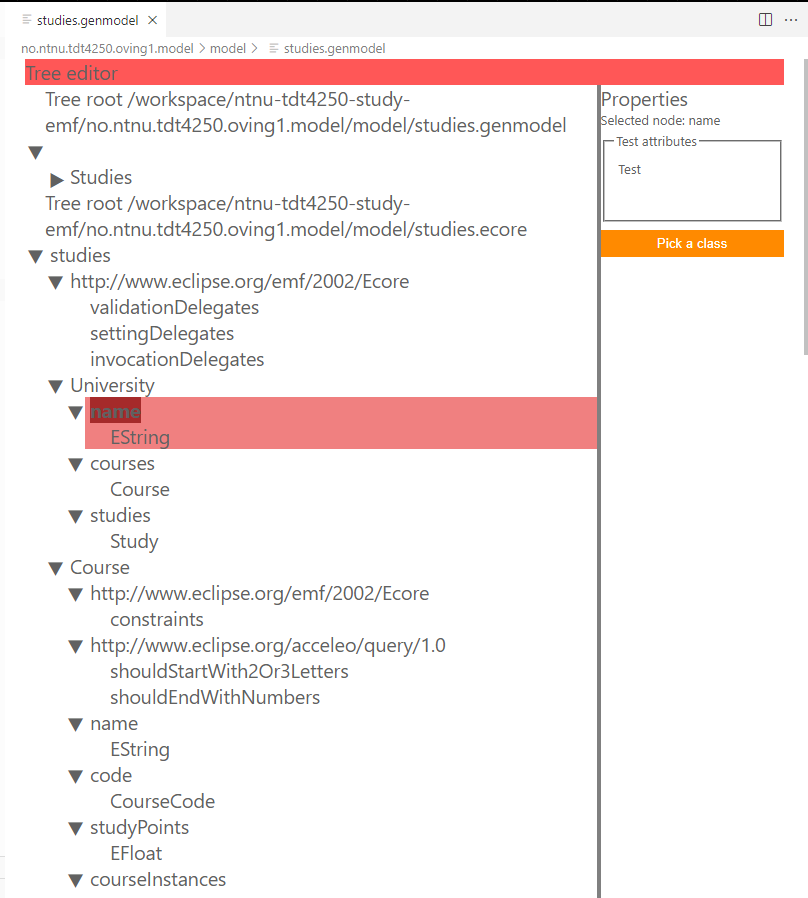
\includegraphics[width=\textwidth]{figures/gitpod-vscode-genmodel.png}
  \caption[Tree Editor Extension showing studies.genmodel]{The Tree Editor Extension with the \texttt{studies.genmodel} file open. It has two roots, the GenModel and the model. The GenModel is collapsed/hidden at the ``Studies'' node.}\label{fig:gitpod-ext-genmodel}
\end{figure}

\begin{figure}[H]  % order of priority: h here, t top, b bottom, p page
  \centering
  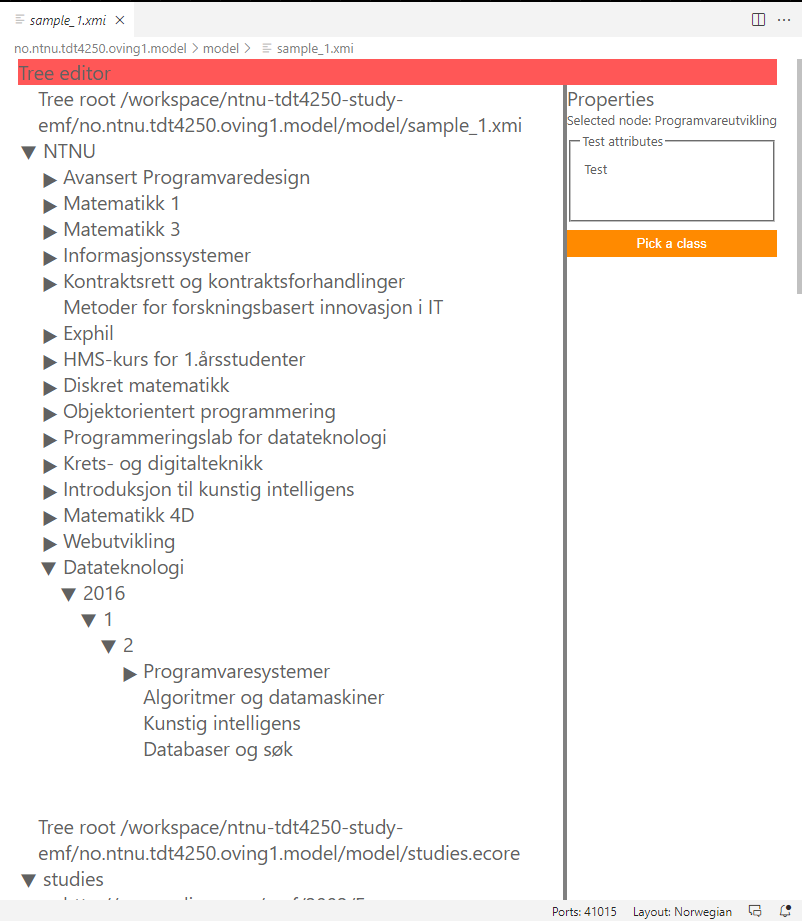
\includegraphics[width=\textwidth]{figures/gitpod-vscode-xmi-study-instance.png}
  \caption[Tree Editor Extension showing a dynamic instance]{The Tree Editor Extension with the \texttt{sample_1.xmi} dynamic instance open. This is data that conforms to the model defined in \texttt{studies.ecore}.}\label{fig:gitpod-ext-dynamic}
\end{figure}


\subsection{Configuration and Logging}

The extension has configuration options that a user can set.
One such option is the logging level, a threshold to hide log messages in the log panel.
The extension can also log internal events and messages to a Output panel in \gls{VSCode}, for the user to debug and identify errors.
The configuration and output panel are shown in \cref{fig:gitpod-ext-config-log}.

\begin{figure}[htbp]  % order of priority: h here, t top, b bottom, p page
  \centering
  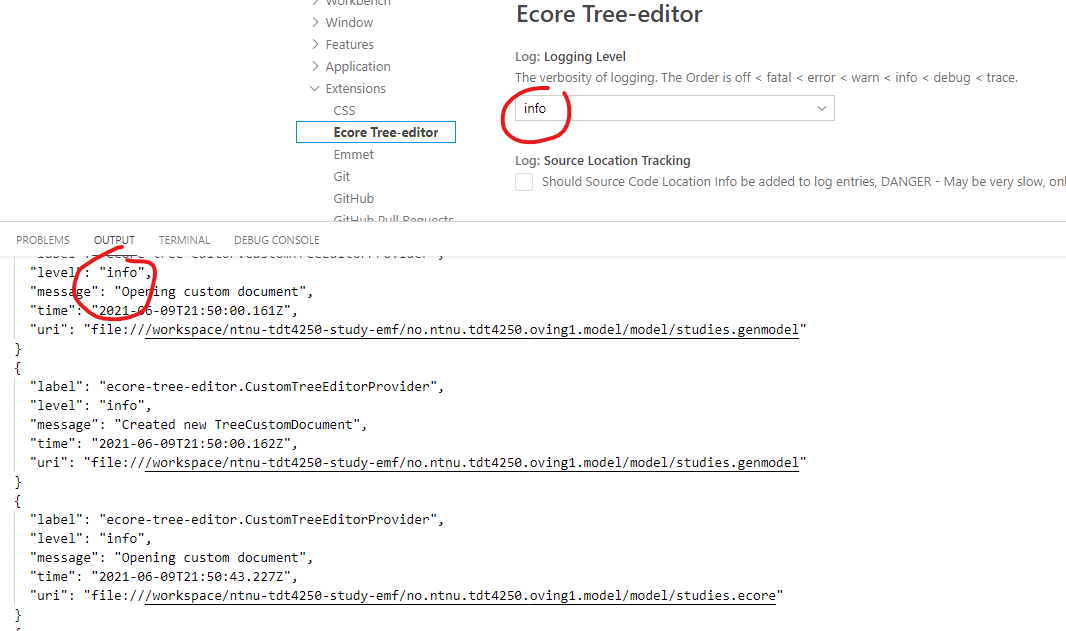
\includegraphics[width=\textwidth]{figures/gitpod-vscode-config-and-logging.png}
  \caption[Tree Editor Extension with configuration and logging]{The Tree Editor Extension adds configuration options to the \gls{VSCode} settings menu, shown in the top right.
  The extension also adds log outputs to a Output panel.
  The figure is annotated with two red circles.
  The upper circle is indicating the configuration option to filter the output based on log level.
  The lower circle is highlighting that same log level from a message in the output panel.}\label{fig:gitpod-ext-config-log}
\end{figure}


\iffalse{
% * Steps:
% 1. Sign up to Gitpod.io with GitHub user
% 2. Go to Settings. Set default IDE as VSCode. (It will be the default soon % % https://github.com/gitpod-io/gitpod/issues/3989#issuecomment-822246441)
% 3. Open %https://gitpod.io/#https://github.com/krissrex/ntnu-tdt4250-study-emf % to get a Workspace in gitpod with an EMF project. The Tree Language Server does % not support multi-workspace.
% 4. Build the extension locally to obtain a .vsix file (or download a build from % somewhere)
% 5. Upload the .vsix to the project workspace by drag-and-drop.
% 6. Right-click the .vsix file in VSCode/Gitpod, select "Install Extension VSIX".
% 7. Wait for "Completed installing Ecore Tree-editor extension from VSIX" popup % in bottom right corner.
% 8. Open folder with models: "no.ntnu.tdt4250.oving1.model/model"
% 9. Click model file: "studies.ecore"
% 10. Click genmodel file: "studies.genmodel"
% 11. Click dynamic instance file: "sample_1.xmi"
}
\fi

\FloatBarrier % Prevent figures running into the next section


\section{Design Artifact: Architecture for Tree Language Server Systems}

% TODO

* Architecturally significant requirements
* Architecture iterations
* Final architecture. C4 diagram (context, containers, components, code)

\begin{figure}[htbp]  % order of priority: h here, t top, b bottom, p page
  \centering
  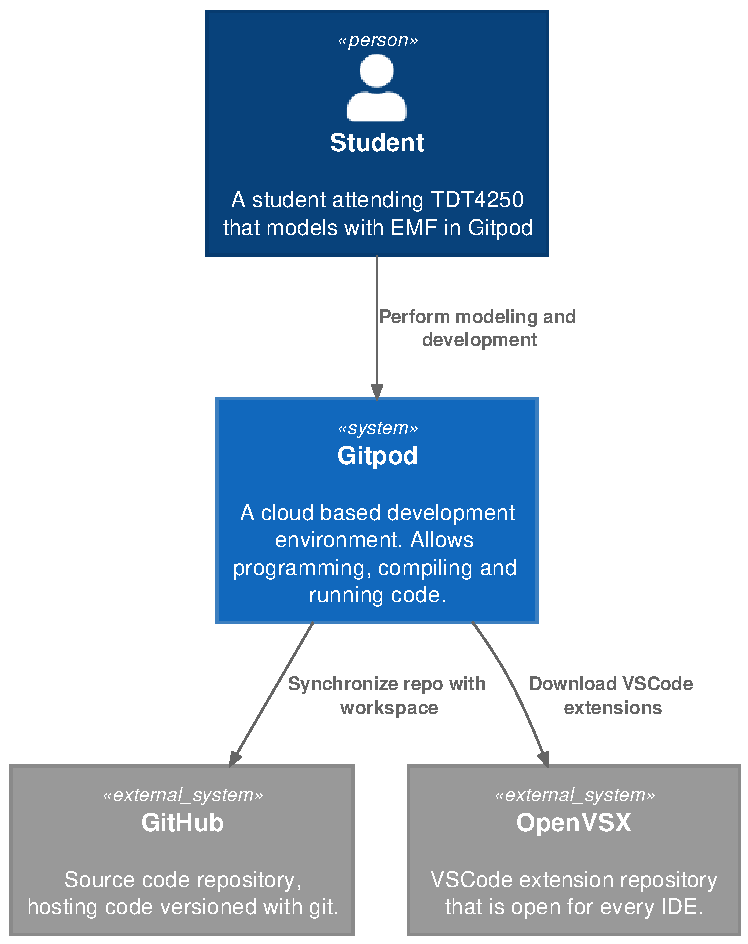
\includegraphics[width=\textwidth]{figures/plantuml/Gitpod_context.pdf}
  \caption[System context diagram for Gitpod]{A system context diagram for Gitpod. The extension will run inside the Gitpod service, used by a student to do modeling and developing. Gitpod uses git to synchronize code with GitHub. The extensions in Gitpod are downloaded from a service called OpenVSX.}\label{fig:gitpod-system-context}
\end{figure}

\begin{figure}[htbp]  % order of priority: h here, t top, b bottom, p page
  \centering
  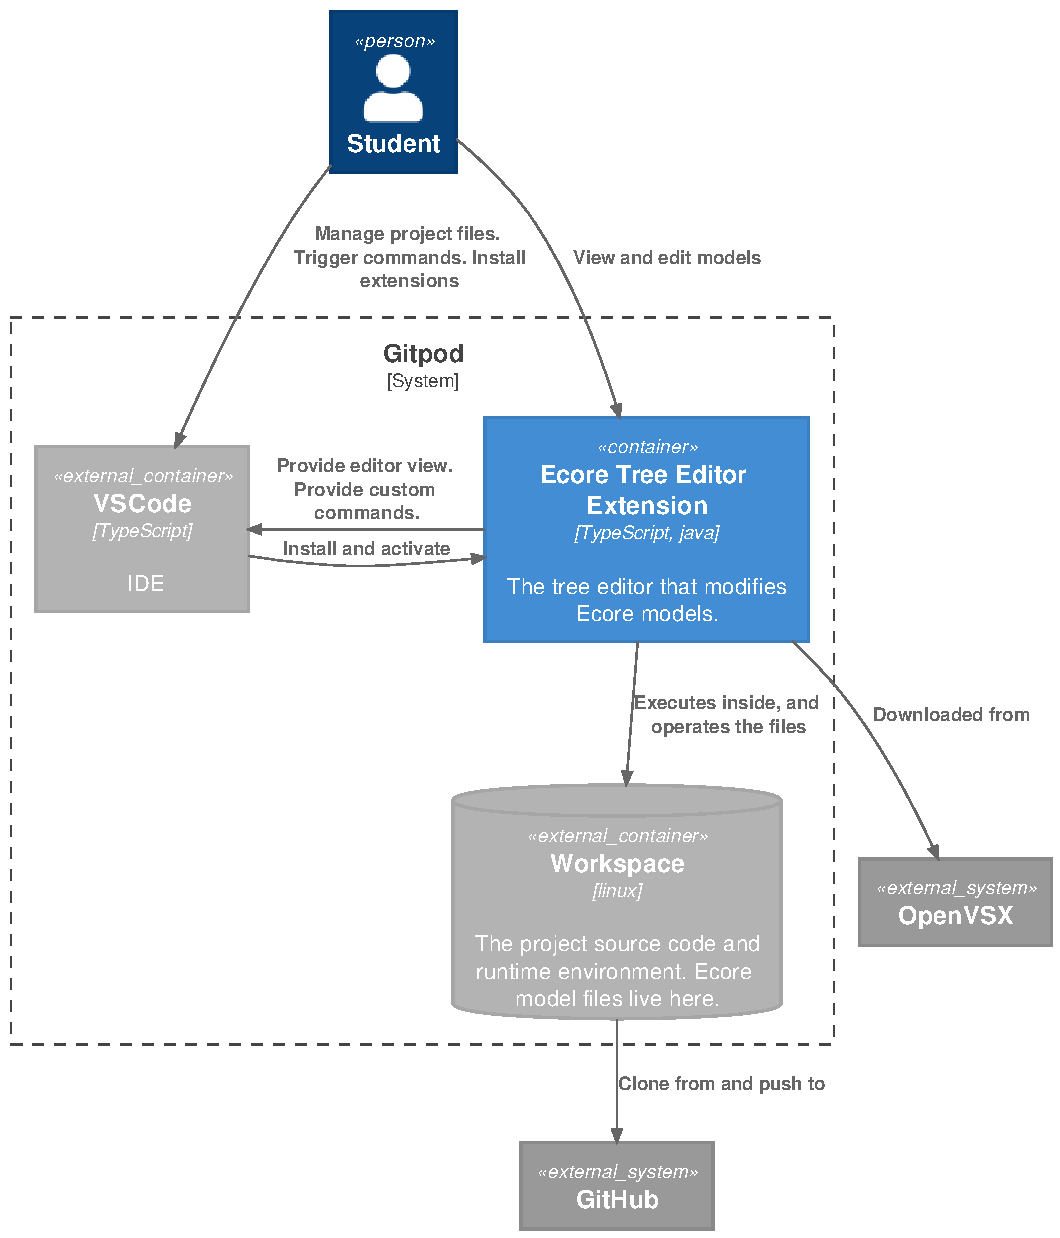
\includegraphics[width=\textwidth,height=\textheight,keepaspectratio]{figures/plantuml/Tree_Editor_Extension_container.pdf}
  \caption[Gitpod container diagram]{Container diagram for gitpod. The Gitpod system from \cref{fig:gitpod-system-context} is expanded to show its internal components. The \acrshort{IDE} used by Gitpod is \gls{Theia}.
  The student will interact with Theia, and install the Ecore Tree Editor Extension created from this thesis.
  This extension will also provide a user interface, which the student uses for modeling.
  This extension reads files from the Gitpod workspace, and uses the runtime provided by the workspace such as a Java Runtime Environment.}\label{fig:gitpod-container-diagram}
\end{figure}

\begin{figure}[htbp]  % order of priority: h here, t top, b bottom, p page
  \centering
  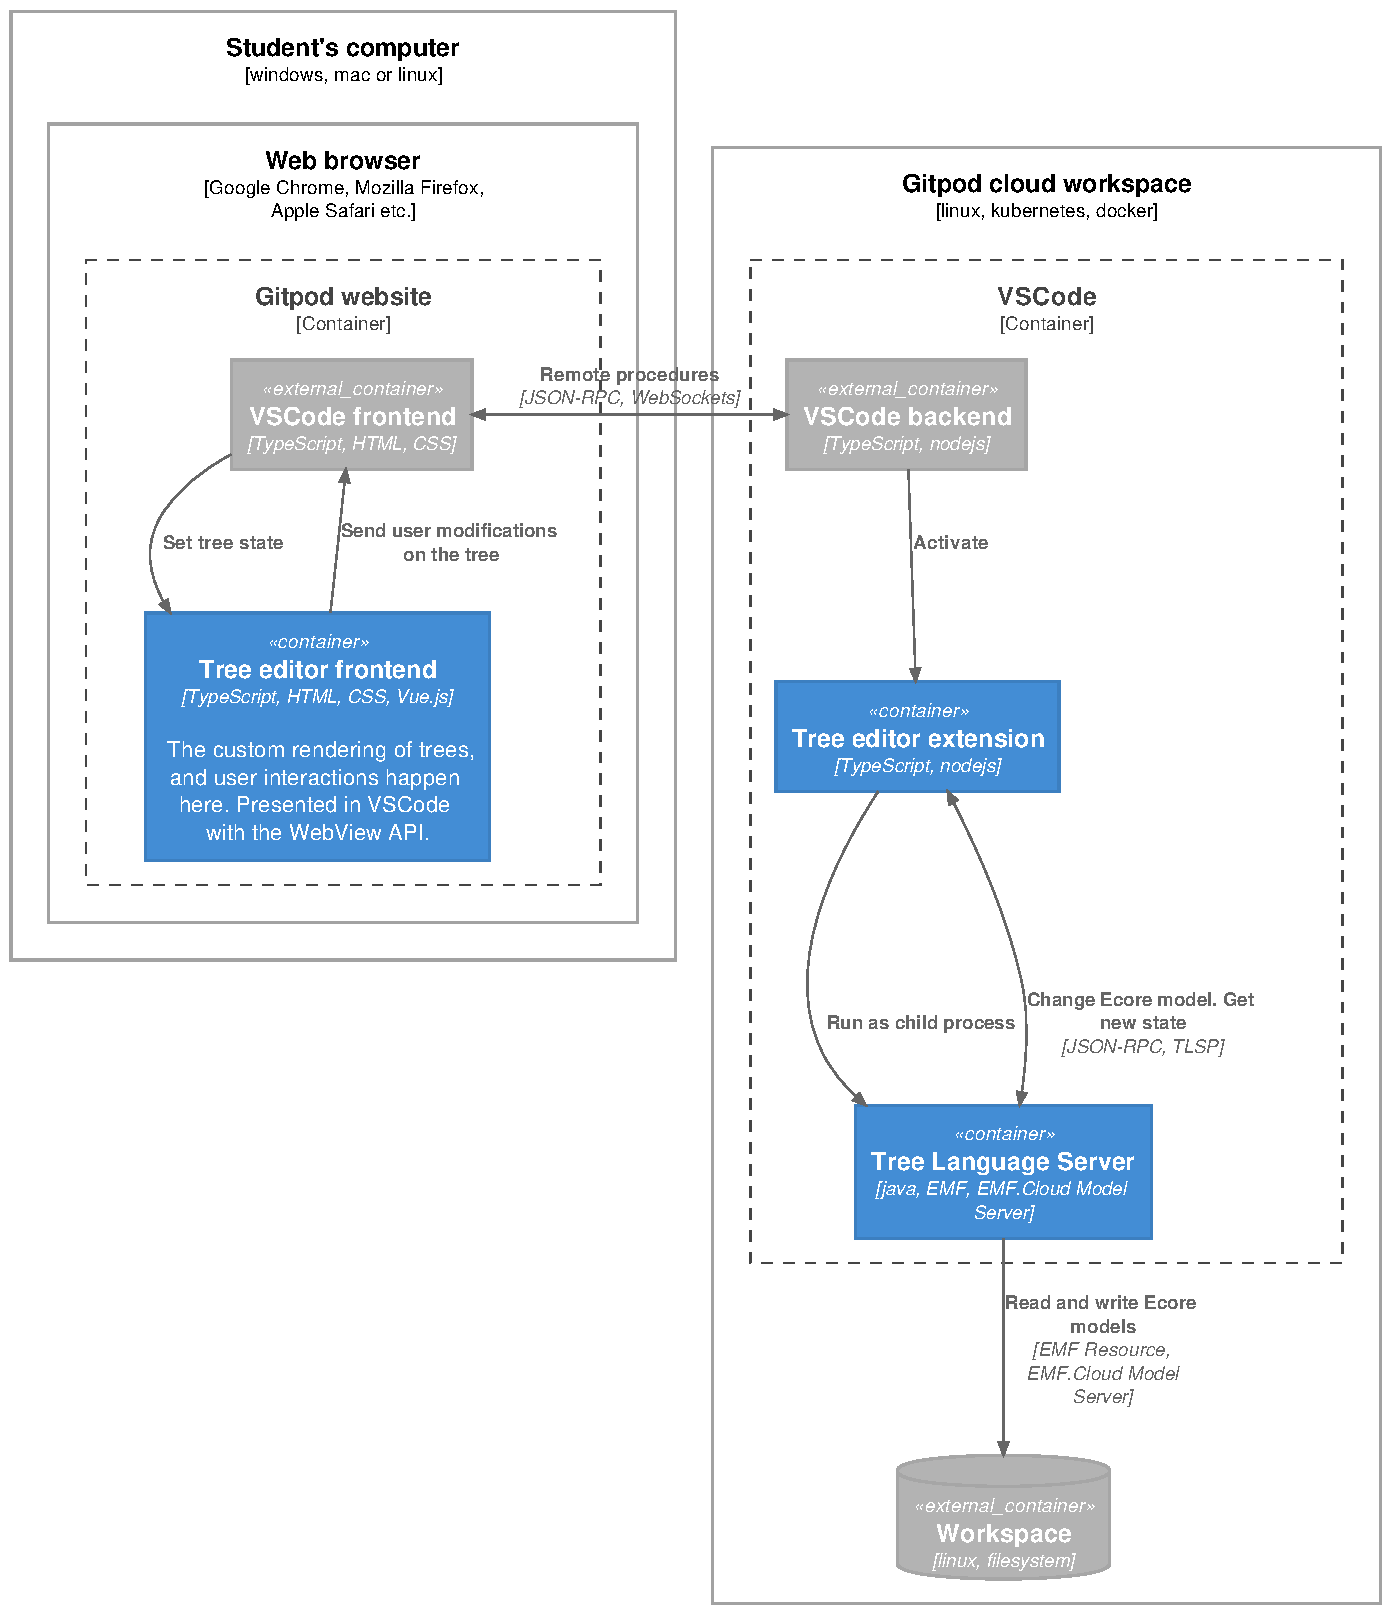
\includegraphics[width=\textwidth,height=\textheight,keepaspectratio]{figures/plantuml/Tree_Editor_Extension_deployment.pdf}
  \caption[Gitpod deployment diagram]{Deployment diagram of Gitpod. The student will use their computer to load the Gitpod website.
  The Gitpod service will start a computer in a cloud provider, to create a cloud workspace.
  The student only loads the Theia frontend and Tree editor frontend into their browser.
  Theia has a backend which runs inside the Workspace, and communicates to the frontend over WebSockets, using JSON-RPC\@.
  The Theia backend will activate the Tree editor extension, which in turn will start a Tree Language Server.
  This Tree Language Server runs java, and reuses the \acrshort{EMF} tooling.
  The Tree editor extension communicates to the Tree Language Server over a well defined protocol, where it asks to read model files, and execute commands to change the models.
  The Tree Language Server uses the Workspace to read and write \texttt{.ecore} files.}\label{fig:gitpod-deployment-diagram}
\end{figure}

\begin{figure}[htbp]  % order of priority: h here, t top, b bottom, p page
  \centering
  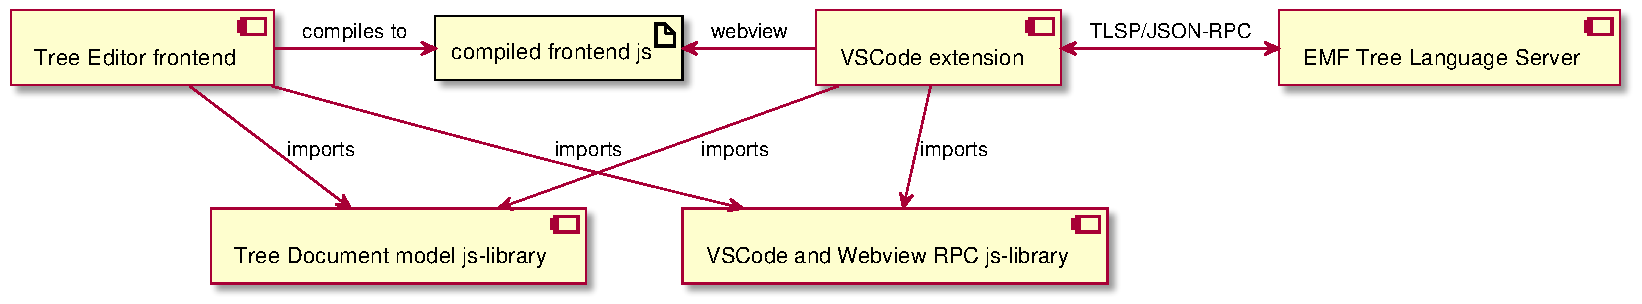
\includegraphics[width=\textwidth]{figures/plantuml/Tree_editor_components.pdf}
  \caption[Ecore Tree Editor component diagram]{Component diagram of the Ecore Tree Editor.
  The for the the extension is organized in 5 separate modules.
  The main module is the VSCode extension.
  This extension bundles the compiled frontend javascript artifact, and the compiled EMF Tree Language Server java jar-file.
  The Tree DOcument model js-library is the layer with the domain model for tree editors.
  It is used in both the frontend and the extension.
  }\label{fig:label4}
\end{figure}


\section{Design Artifact: Tree Language Server Protocol}\label{sec:tlsp}
% TODO



\newcommand{\bluearrowDesc}{The blue half-arrow ($\rightharpoondown$) is part of the \acrfull{TLSP}.}

\begin{figure}[htbp]  % order of priority: h here, t top, b bottom, p page
  \centering
  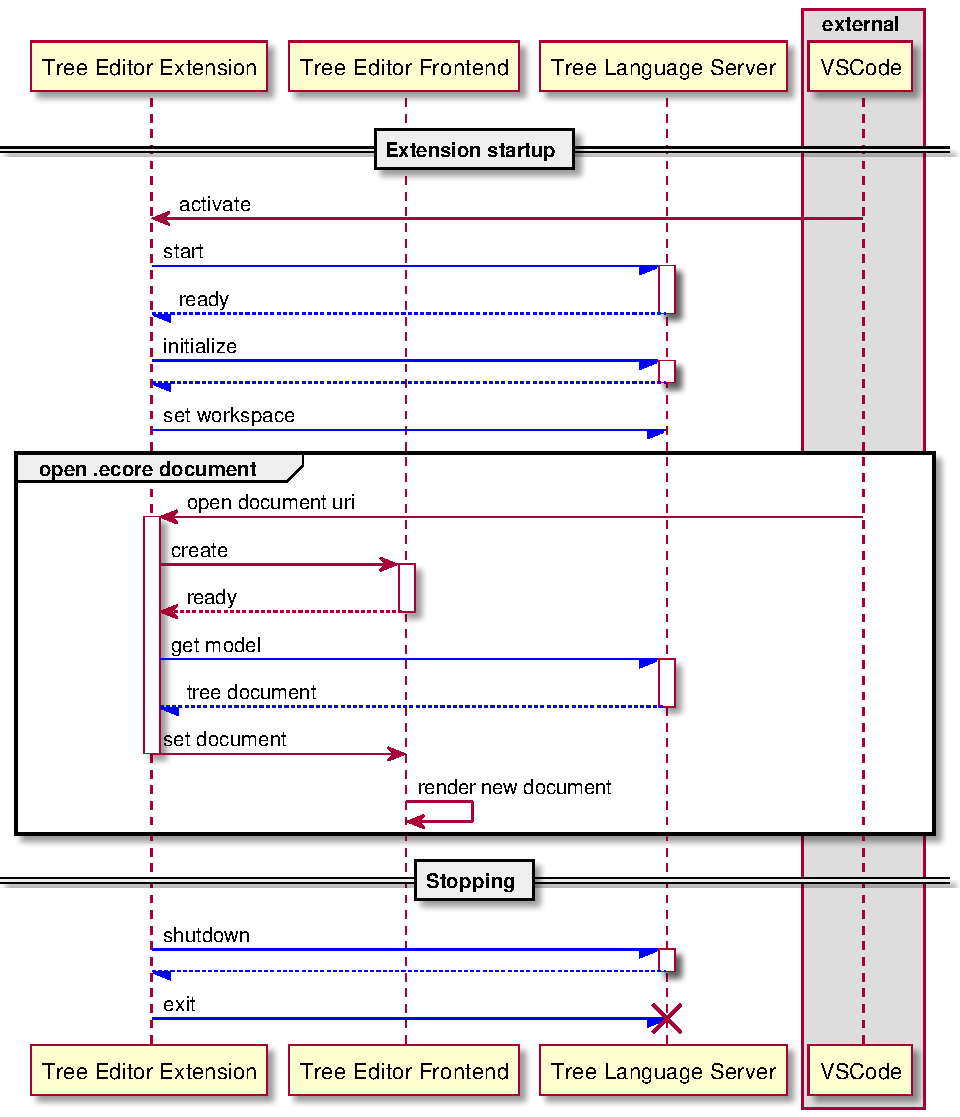
\includegraphics[width=\textwidth]{figures/plantuml/Protocol_startstop_sequence.pdf}
  \caption[Protocol Sequence Diagram of Start/Stop]{Sequence diagram for the protocol when starting and stopping the server. \bluearrowDesc}\label{fig:protocol-startstop}
\end{figure}

\begin{figure}[htbp]  % order of priority: h here, t top, b bottom, p page
  \centering
  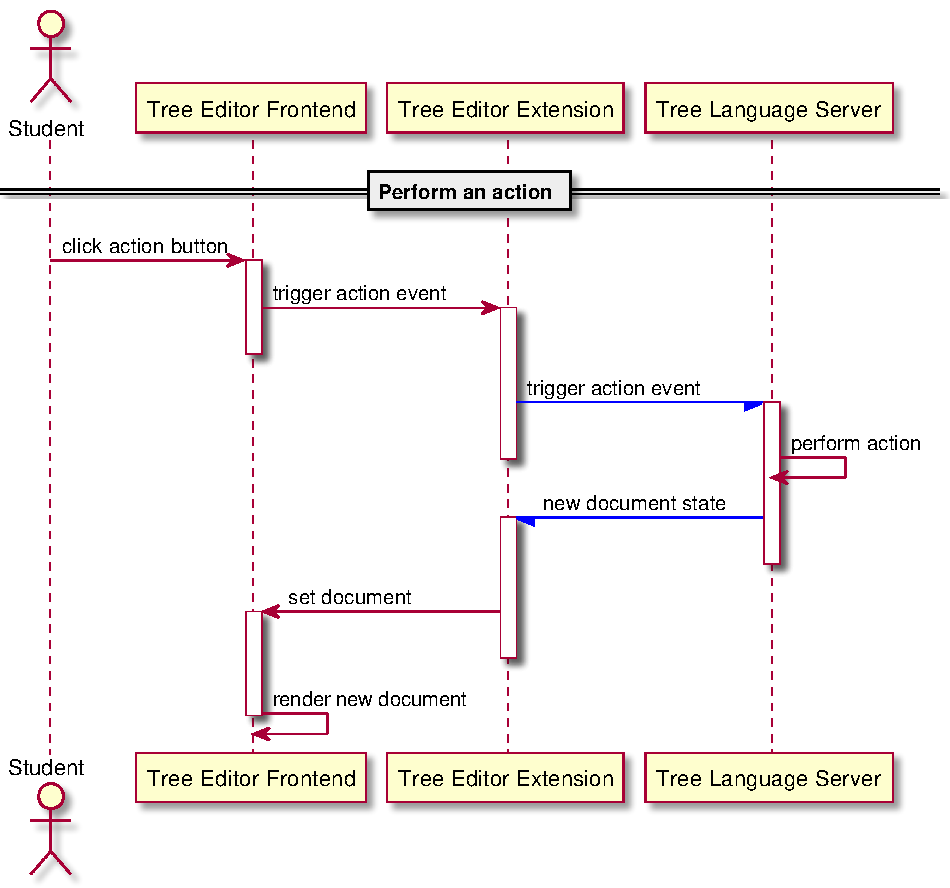
\includegraphics[width=\textwidth]{figures/plantuml/Protocol_action_sequence.pdf}
  \caption[Protocol Sequence Diagram of Action Triggering]{Sequence diagram for the protocol when triggering an action. \bluearrowDesc}\label{fig:protocol-action}
\end{figure}

\begin{figure}[htbp]  % order of priority: h here, t top, b bottom, p page
  \centering
  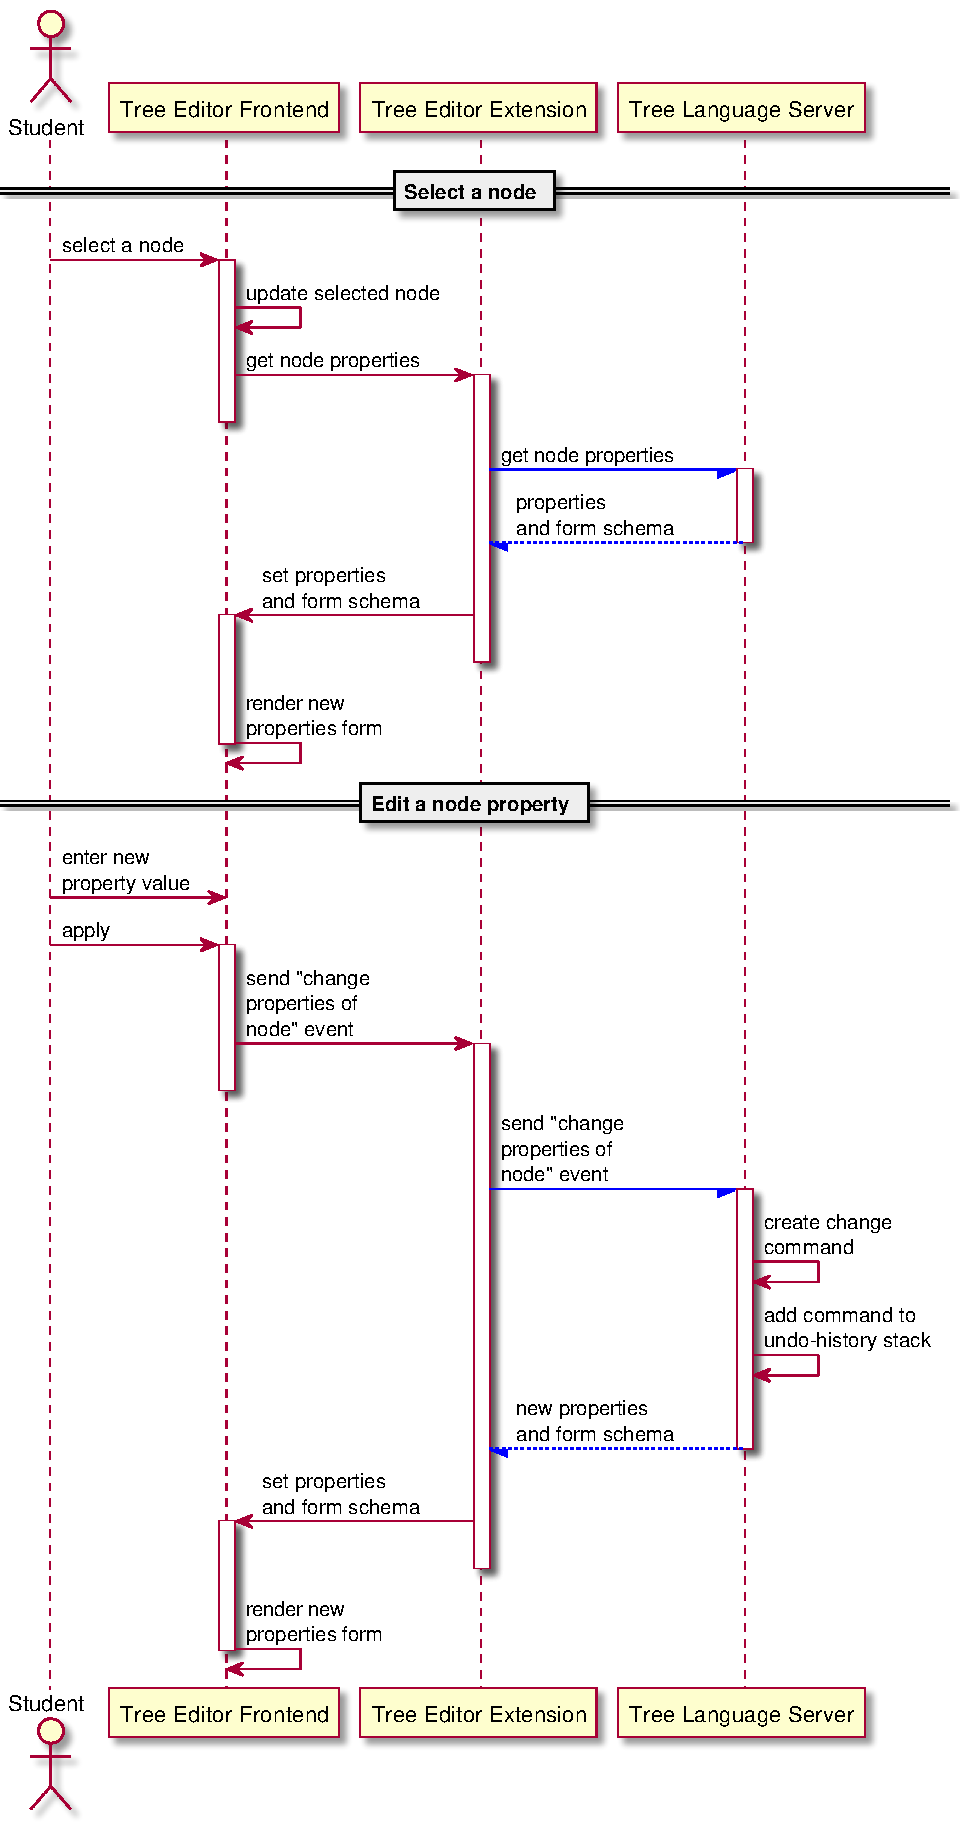
\includegraphics[width=\textwidth,height=\textheight,keepaspectratio]{figures/plantuml/Protocol_form_sequence.pdf}
  \caption[Protocol Sequence Diagram of Property Form]{Sequence diagram for the protocol when editing a node property. \bluearrowDesc}\label{fig:protocol-form}
\end{figure}

\begin{figure}[htbp]  % order of priority: h here, t top, b bottom, p page
  \centering
  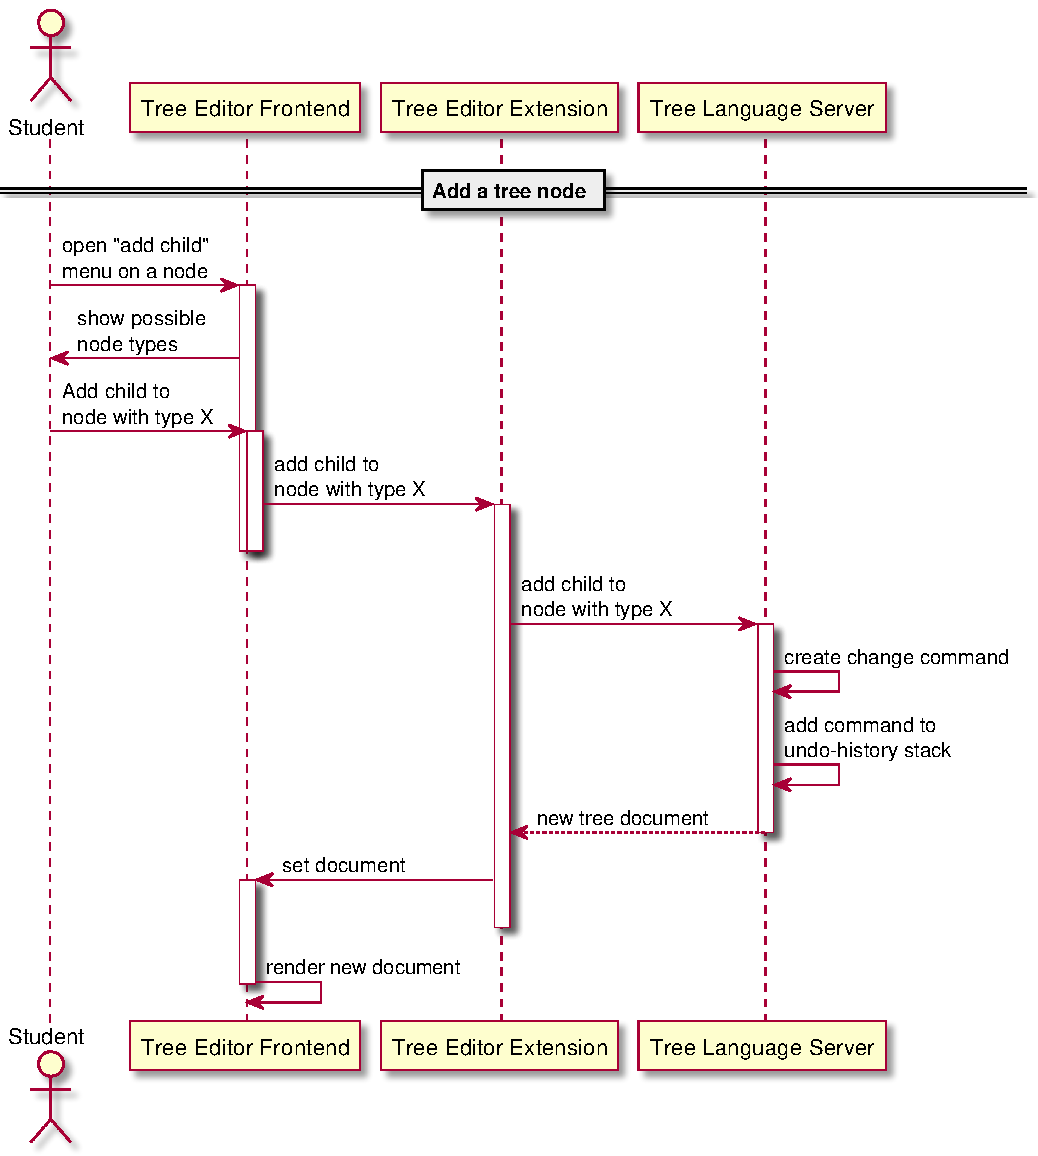
\includegraphics[width=\textwidth]{figures/plantuml/Protocol_changetree_sequence.pdf}
  \caption[Protocol Sequence Diagram of Tree Changes]{Sequence diagram for the protocol when adding a child node. \bluearrowDesc}\label{fig:protocol-changetree}
\end{figure}

\FloatBarrier


* TLSP protocol. JSON-RPC based with LSP Base, with a Tree Document Model data structure. Hierarchy schemas for optimistic-view drag-n-drop. Type and id based nodes. 


\section{Open Source Project: Measures Taken for Viability and Maintainability}
% TODO

* A project that may be viable and further developed.
  * Bundled IDE configuration: recommended extension, build tasks, run configurations. Reduces overhead for new developers.
  * NOT: CI/CD. Easily added later when needed. Overhead for 1-man project.
  * Build-scripts and npm/maven for building.
  * Readme-files for all components and modules.
  * Commonly used programming languages and (official) dependencies
  

\chapter{Evaluation}\label{chap:evaluation}

% TODO

\section{Test of Value for Students from Tree Editor}

* Feature test based on Confluence tasks.
  * Result: missing many features still. Not usable in education.

\section{Test of Value for Extension Developers from Protocol}
* Protocol-to-usecase parity. (Protocol-to-emfCommands parity?)
  * Result: JSON-RPC part is missing most features still. Not stable and recommended for adoption. The extension needs more features in order to grow the protocol. The data structure is valid; it can represent different tree structures from domains like Ecore, json and file systems.

\section{Acceptance Test of Tree Editor Extension}

\subsection{Runtime Environment Test}
* Environment end-to-end test in gitpod.
  * Result: the extension can install and render Ecore diagrams.

\subsection{Flexibility Test}
* Flexibility test to change the label or which properties are shown as children.
  * Result: failed. No such feature yet. No major blocker except development time.

\subsection{Functionality Test}
* Editor functionality test.
  * Result: Can view multiple trees and select nodes. Can show/hide children. Does not show correct icon. Missing drag-and-drop, editing, keyboard shortcuts, right click, keyboard navigation, validation.

\subsection{Test of Viability of Open Source Project}
* Project viability test.
  * Result: has a good kernel. Missing issues and roadmap on github. Clean code, but many TODO/FIXME that are unresolved. 
  
\chapter{Discussion}\label{chap:discussion}

% TODO

* Uncertain if the LSP or GLSP has the best approach (many vs few procedures, action handler, message-relaying)

* Some ideas of LSP are not carried on, like "capability querying". Is it needed? Agile says not yet (YAGNI).

* Suggestions to how the protocol should look or be developed.

* Is the method correct?

* Can the evaluation be trusted?

* Is a tree editor the correct thing to build? EMF adoption may be hindered by:
  * Bad or missing documentation+guides+examples
  * Missing genmodel towards web (typescript. cross-ecore tries to address this, but is not stable yet and not configurable with genmodel)
  * Generated Ecore java API is cumbersome, unintuitive, poorly documented, not fluent.
  * Ecore is too oriented towards Eclipse as the runtime, with Eclipse specific Design Patterns (Adapter, ItemProvider etc).
\chapter{Conclusion}\label{chap:conclusion}

This thesis started by finding a way to enable modeling using \acrlong{EMF} in the \gls{cloud}, to solve Objective 1.
A pre-project suggested creating a tree editor for \gls{Gitpod}, by creating a \gls{VSCode} extension.
This thesis then designed an extension which used a software architecture and protocol that drew inspiration from the \acrlong{LSP} and \acrlong{GLSP} designs.
The thesis also presented a way to implement a tree editor with this architecture, and a method which extracts functional requirements from the existing \acrshort{EMF} tree editors in \gls{Eclipse} through use cases.
The architecture is a three component system: a generic tree editor frontend, a \gls{VSCode} extension, and an \acrshort{EMF}-specific server.
This architecture also entailed using a protocol, dubbed the \acrfull{TLSP}, between the \gls{VSCode} extension and the server.
This design was implemented up to the point it could successfully render \acrshort{EMF} models in \gls{Gitpod} with \gls{VSCode}.\\

The successful design and implementation of this architecture means it can be the basis of a new sibling protocol to \acrshort{LSP} and \acrshort{GLSP}: the \acrshort{TLSP}.
This can be used by other tools that undergo a similar migration to the \gls{cloud}. 
This design also created encapsulated and reusable components.
It can also ease future migration of \acrshort{EMF} to another \acrlong{IDE}, because the \acrshort{EMF} logic is contained in a reusable server, independent of \gls{VSCode}.
This means it solves Objective 3: An architecture to enable future related IDE migrations.\\

Lastly, this thesis produced an \gls{open source} project for the editor and \acrshort{TLSP}.
However, open sourcing software requires more effort than what is currently done to attract contributions.
Gaining traction online for \gls{open source} is similar to product marketing.
The amount of effort required to create a viable solution for \gls{cloud} based tree editing in \gls{VSCode} is substantial.
External contributions may be required for completing the implementation.



\section{Future Work}

This thesis has uncovered some new potential areas of research.

\paragraph{Theia or VSCode as a deployment platform}
The GenModel and code generator can target \gls{Eclipse} as a deployment platform.
The model gets a plugin generated, and an editor in \gls{Eclipse} for model instances.
A similar approach can be interesting for deploying a tree editor for model instances, but using \gls{Theia} or \gls{VSCode} instead of \gls{Eclipse}.
These could potentially reuse the \acrshort{TLSP} as well.
Doing this would increase the value of \acrshort{EMF}, and further illustrate the values of \acrlong{MDD} and code generation.

\paragraph{Collaborative modeling}
Modeling is a collaborative task.
With the move to cloud, and with the increased amount of work from home\footnote{Due to covid-19.}, collaboration can move online as well.
This is already normal for things like Google Docs, and Jetbrains just added ``Code With Me''.
Obeo is also developing this for their cloud based Sirius modeling tool.
When all the editing is done through a protocol like \acrshort{TLSP}, the data could be redirected to multiple clients, meaning multiple students' computers.

\paragraph{Completing the EMF editor}
A lot of the remaining work is routine design, not research.
But some remaining parts may be more challenging, such as getting the GenModel working and specializing the editor to properly show a \texttt{.genmodel} file like in \gls{Eclipse}.
There are also challenges to loading the generated code back into the server, for validations and custom \texttt{ItemProviders}.
Completing this will make the editor more useful, and also move it closer to a solution suited for industry use, beyond just education.




\chapter*{\bibname}
\printbibliography[heading=none]

\appendix
\chapter{Tree Editor Functional Requirements from Pre-project}\label{app:functional-requirements}

The following \cref{tab:function-requirements} is copied from the results section in the pre-project, at \cite[p.~47-48]{rekstadModelingEnvironmentCloud2020}.
It presents a non-complete list of functional requirements for a tree editor.

% Please add the following required packages to your document preamble:
% \usepackage{longtable}
% Note: It may be necessary to compile the document several times to get a multi-page table to line up properly
\begin{longtable}{lp{3cm}p{6cm}}
\caption{Functional requirements for a master-detail Tree editor with property sheet.}
\label{tab:function-requirements}\\
\multicolumn{1}{c}{\textbf{ID}} &
  \multicolumn{1}{c}{\textbf{Requirement}} &
  \multicolumn{1}{c}{\textbf{Description}} \\ \hline
\endfirsthead
%
\multicolumn{3}{c}%
{{\bfseries Table \thetable\ continued from previous page}} \\
\multicolumn{1}{c}{\textbf{ID}} &
  \multicolumn{1}{c}{\textbf{Requirement}} &
  \multicolumn{1}{c}{\textbf{Description}} \\ \hline
\endhead
%
FR1 &
  Provide an interactive Tree Editor in VSCode and Theia (Gitpod) &
  \begin{tabular}[c]{@{}p{6cm}@{}}The software must use an extension mechanism to provide a custom editor for trees.\\ A textual representation is not sufficient.\\ The tree comprises a hierarchy of nodes and their child nodes.\end{tabular} \\
FR2 &
  Provide an interactive Property sheet in VSCode and Theia (Gitpod) &
  \begin{tabular}[c]{@{}p{6cm}@{}}The software must use an extension mechanism to provide a custom property sheet for tree nodes.\\ The property sheet needs to be synchronized with the selected node in the tree editor.\end{tabular} \\
FR3 &
  Provide an action bar with dynamically provided actions in VSCode and Theia (Gitpod). &
  The action bar should have actions that are specified by a backend Tree Language Server. \\
FR4 &
  The Tree must view nodes with labels and icons. &
  \begin{tabular}[c]{@{}p{6cm}@{}}Every node should have a default icon that depends on its node "type".\\ Every node should have a name that is read from the node data.\end{tabular} \\
FR5 &
  Tree nodes with children can toggle the visibility of children by user interaction. &
  \begin{tabular}[c]{@{}p{6cm}@{}}An icon or symbol will show if a node has children.\\ If the user interacts with this icon, e.g. a click, all the children will toggle their visibility on/off.\end{tabular} \\
FR6 &
  The Tree and Property views update automatically when the underlying model changes. &
  Subscribe to change notifications from the Model Server, in the Tree Language Server. \\
FR7 &
  The Action Bar updates when the tree selection changes. &
  Show the available actions for the newly selected node. \\
FR8 &
  Support creation of new nodes. &
   \\
FR9 &
  Support deletion of existing nodes. &
   \\
FR10 &
  Support selecting a node. &
   \\
 &
   &
  
\end{longtable}
\chapter{Pre-project Data Structure Code}\label{app:pre-project-tree-structure}

The data structure for containing a tree, designed in the pre-project during prototype number two, is shown in \cref{lst:prototype2-node-tree}.\\

The structure for Actions are shown in \cref{lst:prototype2-action-list} and \cref{lst:prototype2-action-schema}.\\

The structure for defining a node hierarchy is shown in \cref{lst:prototype2-hierarchy-schema}.

\lstinputlisting[
    caption={Javascript code from the WebView for a data model describing the tree nodes. This listing is copied from ``Code listing 5.3'' in~\cite[p.43,44]{rekstadModelingEnvironmentCloud2020}.},
    label=lst:prototype2-node-tree,
    language=JavaScript
]{listings/pre-project/node-tree.js}

\lstinputlisting[
    caption={Javascript code from the WebView to specify the available actions.
    This listing is copied from ``Code listing 5.4'' in~\cite[p.45]{rekstadModelingEnvironmentCloud2020}.},
    label=lst:prototype2-action-list,
    language=JavaScript
]{listings/pre-project/available-actions.js}

\lstinputlisting[
    caption={Javascript code from the WebView to specify default actions and per-node actions.
    This listing is copied from ``Code listing 5.5'' in~\cite[p.45]{rekstadModelingEnvironmentCloud2020}.},
    label=lst:prototype2-action-schema,
    language=JavaScript
]{listings/pre-project/action-schema.js}


\lstinputlisting[
    caption={Javascript code from the WebView to specify what children a node type can have.
    This listing is copied from ``Code listing 5.6'' in~\cite[p.45]{rekstadModelingEnvironmentCloud2020}.},
    label=lst:prototype2-hierarchy-schema,
    language=JavaScript
]{listings/pre-project/hierarchy-schema.js}
%\input{appendices/a-appendix.tex}

\end{document}
